\chapter{L'intelligenza}
La fase di costruzione dell'intelligenza che dovrebbe permettere di comprendere quando vengono suonate le note in una traccia audio si è divisa in due fasi. La prima è stata quella di riconoscere la differenza tra nota e non nota dati dei audio selezionati manualmente senza considerare la lunghezza. In un secondo momento si è poi proceduto dividendo i campioni di note in più parti di uguale lunghezza, associando a ogni divisione del campione un valore che va da 1 a 5, ovvero delle classi che indicano, essere certamente una nota associandovi la classe 5, o essere certamente non una nota accoppiando il campione alla classe 1.\\
Le tracce di strumenti fornitemi dal tutore e utilizzate per gli esperimenti sono state quelle di: 
\begin{itemize}
	\item Contrabbasso
	\item Rullante spazzolato
	\item Colpo di rullante
	\item Colpo di cassa
\end{itemize}


\section{Prima fase}
In questa fase lo scopo è stato appunto comprendere se una macchina con le features selezionate è in grado di riconoscere la differenza tra nota e non nota. Una volta creato il file ARFF contenente le informazioni necessarie tramite un apposito script python lo stesso file è stato usato per costruire l'albero decisionale utilizzando l'algoritmo J48 (versione più fine di ID3 descritto nel Capitolo 2) ottenendo come risultato le matrici di confusione\footnote{Le colonne di queste matrici di confusione indicano il valore atteso, sulle righe vi sono invece i valori risultanti} per gli strumenti sopra elencati in figura \ref{fig:cm_1}\\

I campioni da classificare sono stati divisi in due classi: ``si'' e ``no'' identificanti note e non note. Nella tabella \ref{tab:numerosità_1} si può osservare la numerosità di campioni per ogni classe, la classe con meno campioni è quella del colpo di rullante vista la natura delle tracce audio, è stato complesso estrarre dei campioni adatti vista la natura dello strumento e della registrazione, infatti le note erano spesso molto vicini tra loro e confusi oltre che essere molto inferiori rispetto a quelle degli altri strumenti.

\begin{table}[h!]
	\begin{center}
		\begin{tabular}{l|c|r} % <-- Alignments: 1st column left, 2nd middle and 3rd right, with vertical lines in between
			\textbf{Classe} & \textbf{Si} & \textbf{No}\\
			%			$\alpha$ & $\beta$ & $\gamma$ \\
			\hline
			Basso & 121 & 94\\
			Rullante Spazzolato & 80 & 73\\
			Colpo di Rullante & 64 & 73\\
			Cassa & 132 & 72
		\end{tabular}
		\caption{Numerosità campioni prima fase.}
		\label{tab:numerosità_1}
	\end{center}
\end{table}

\begin{figure}[h!]
	\centering
	\begin{subfigure}{.5\linewidth}
		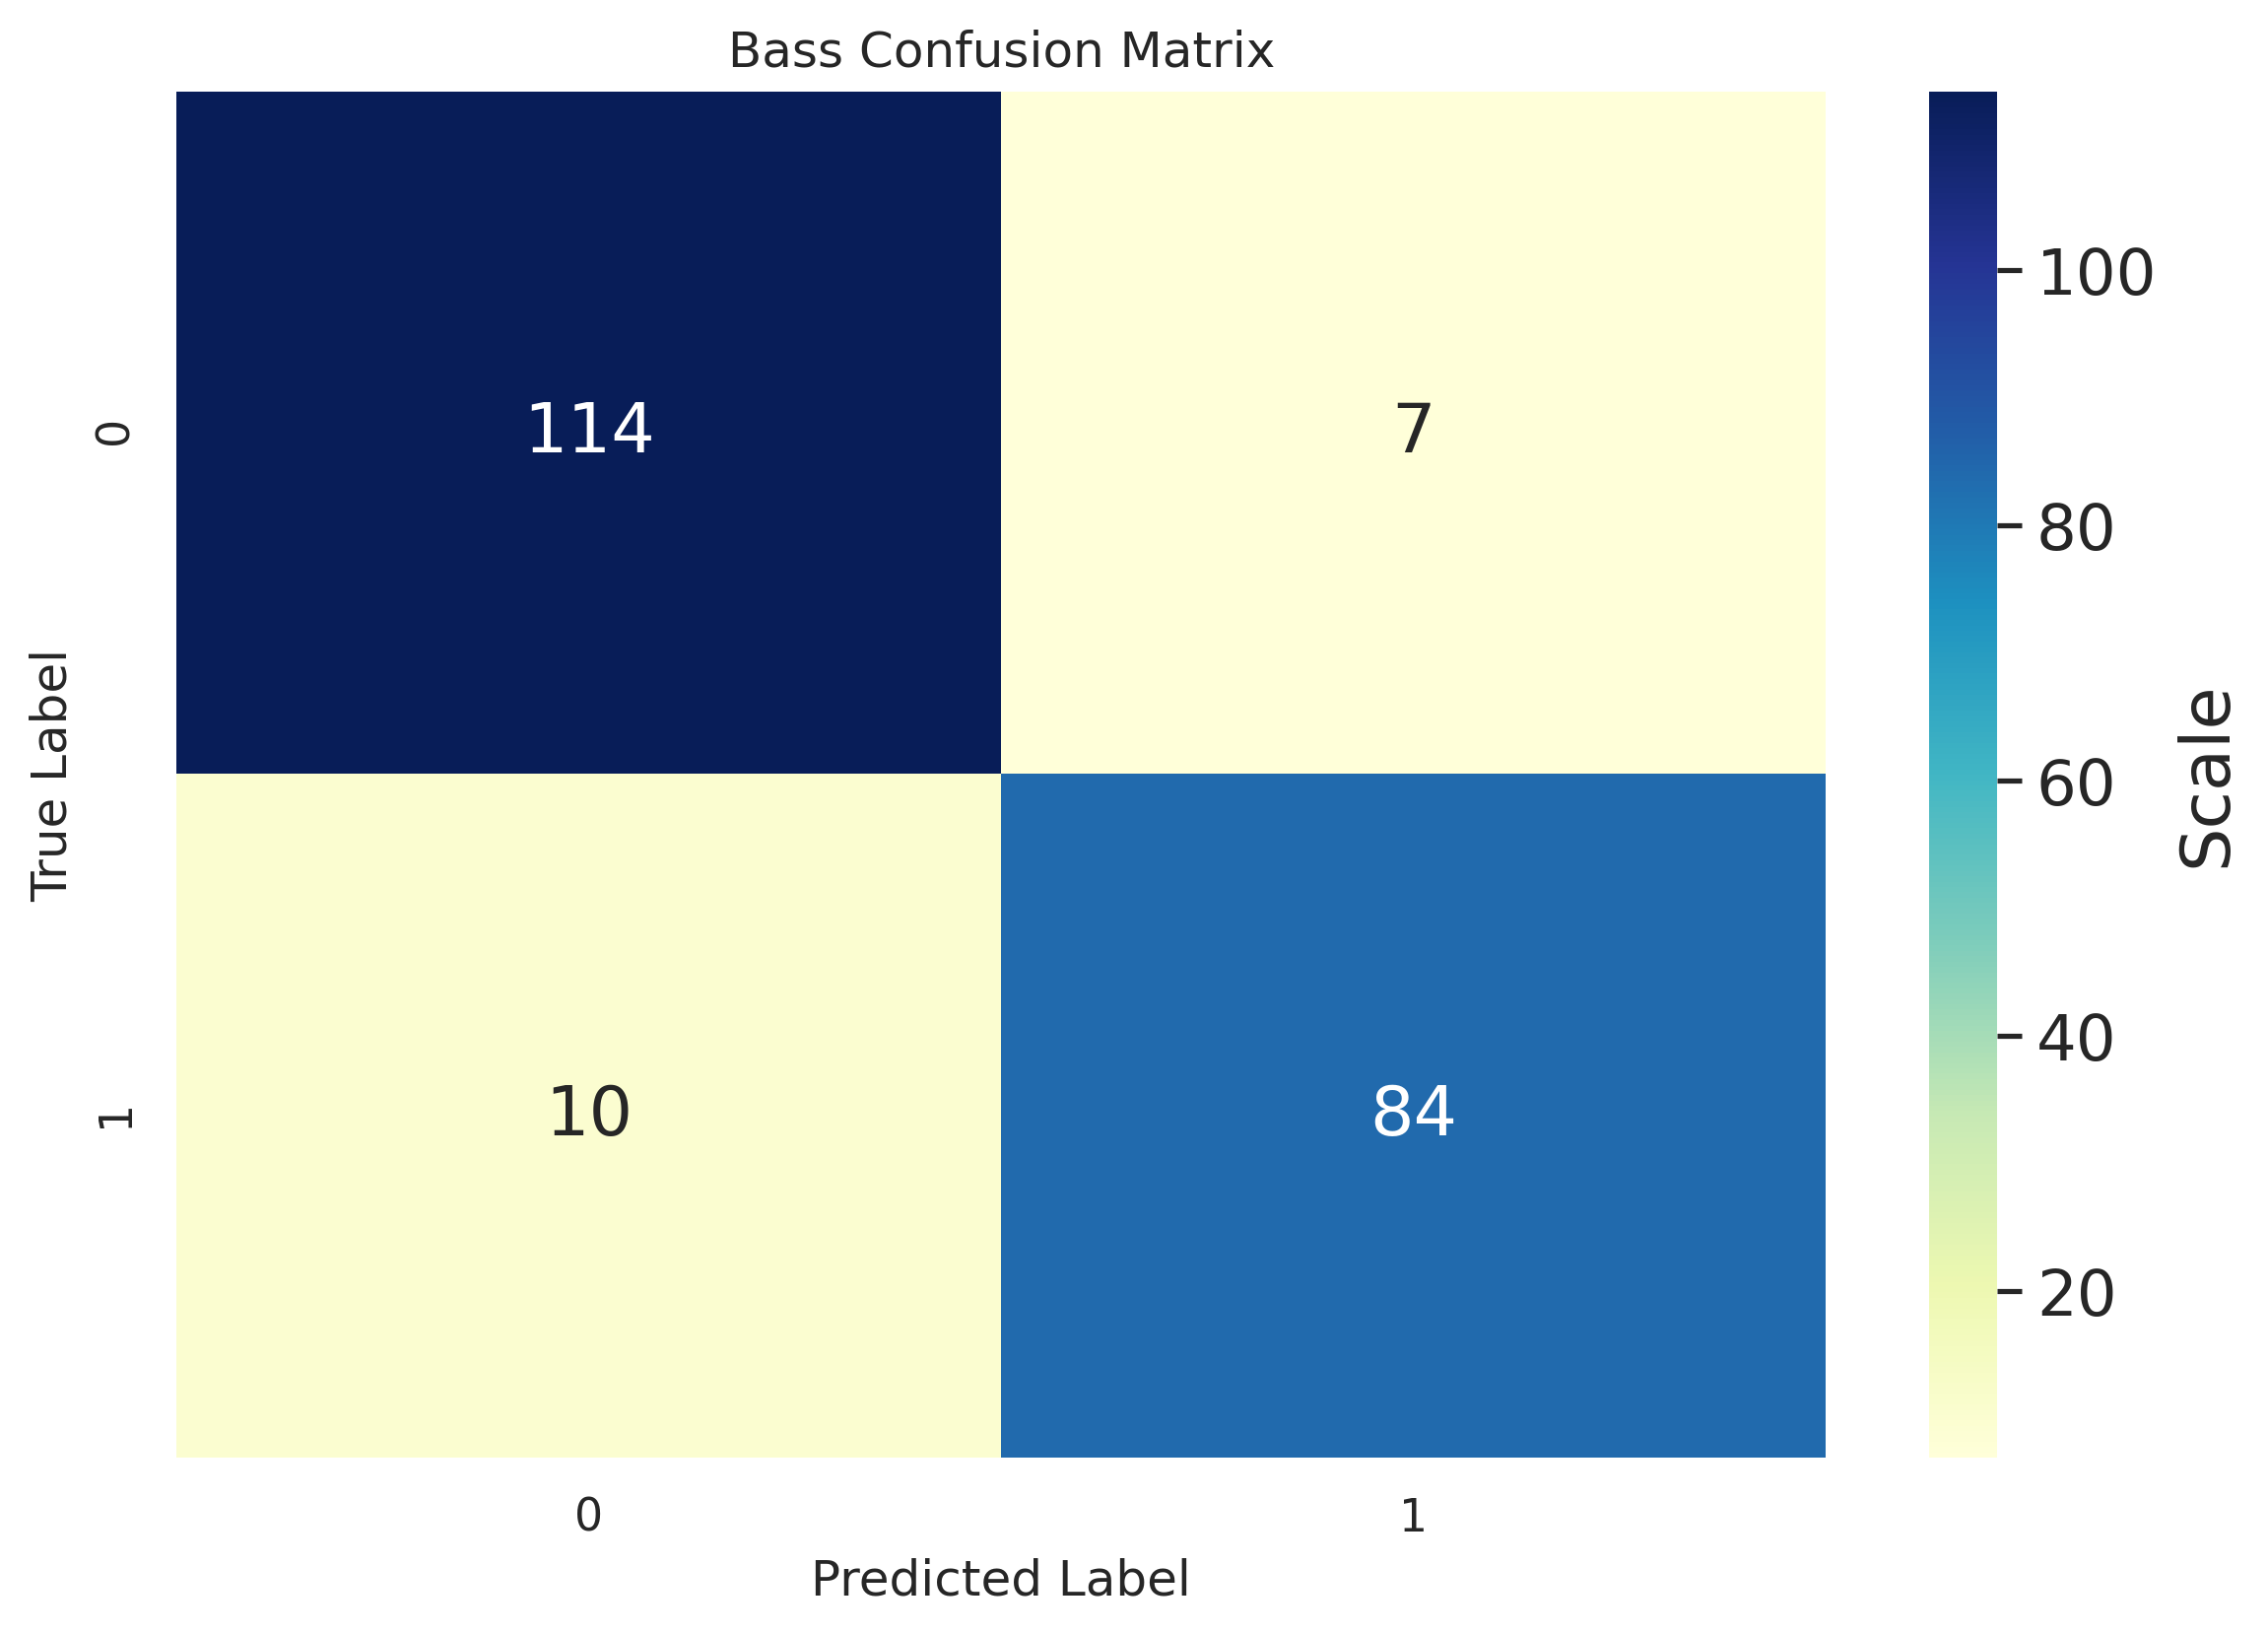
\includegraphics[width=\linewidth]{./immagini/first_classification/cb_cm.png} 
		\caption{Matrice di confusione per il basso}
		\label{fig:cm_1a}
	\end{subfigure}\hfill
	\begin{subfigure}{.5\linewidth}
		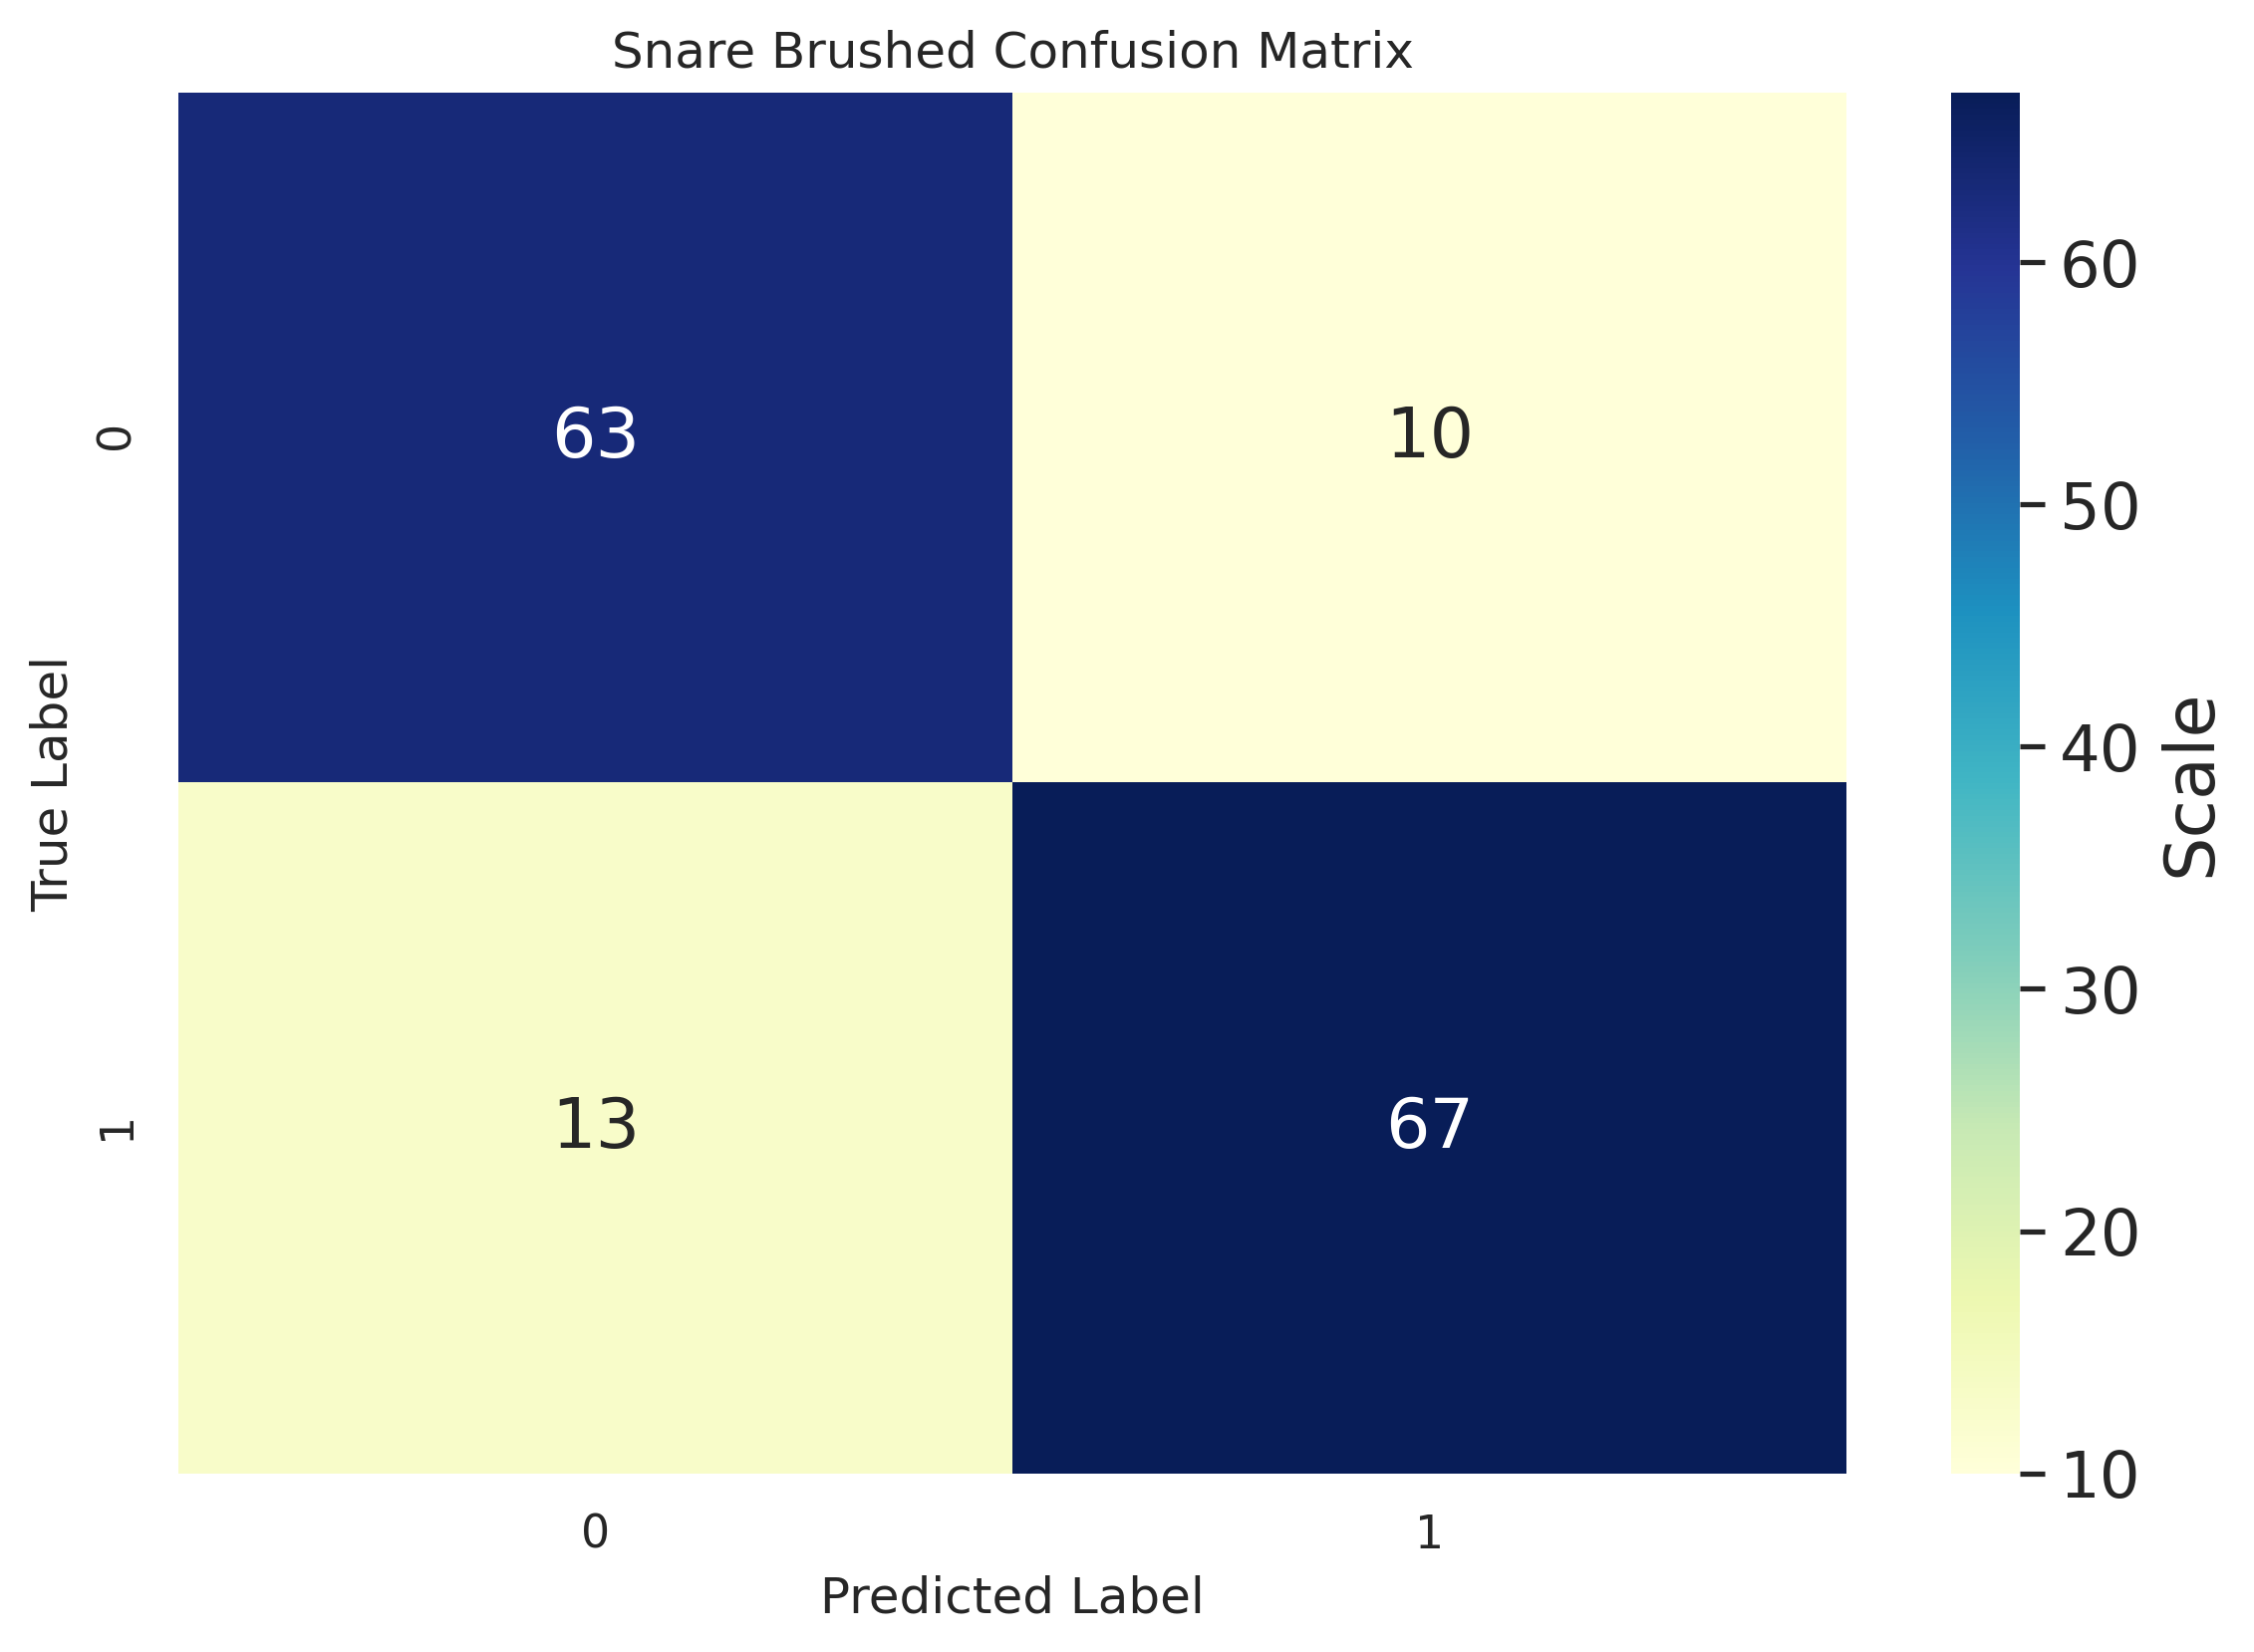
\includegraphics[width=\linewidth]{./immagini/first_classification/sn_brushed_cm.png}
		\caption{Matrice di confusione per il rullante spazzolato}
		\label{fig:cm_1b}
	\end{subfigure}
	
	\begin{subfigure}{.5\linewidth}
		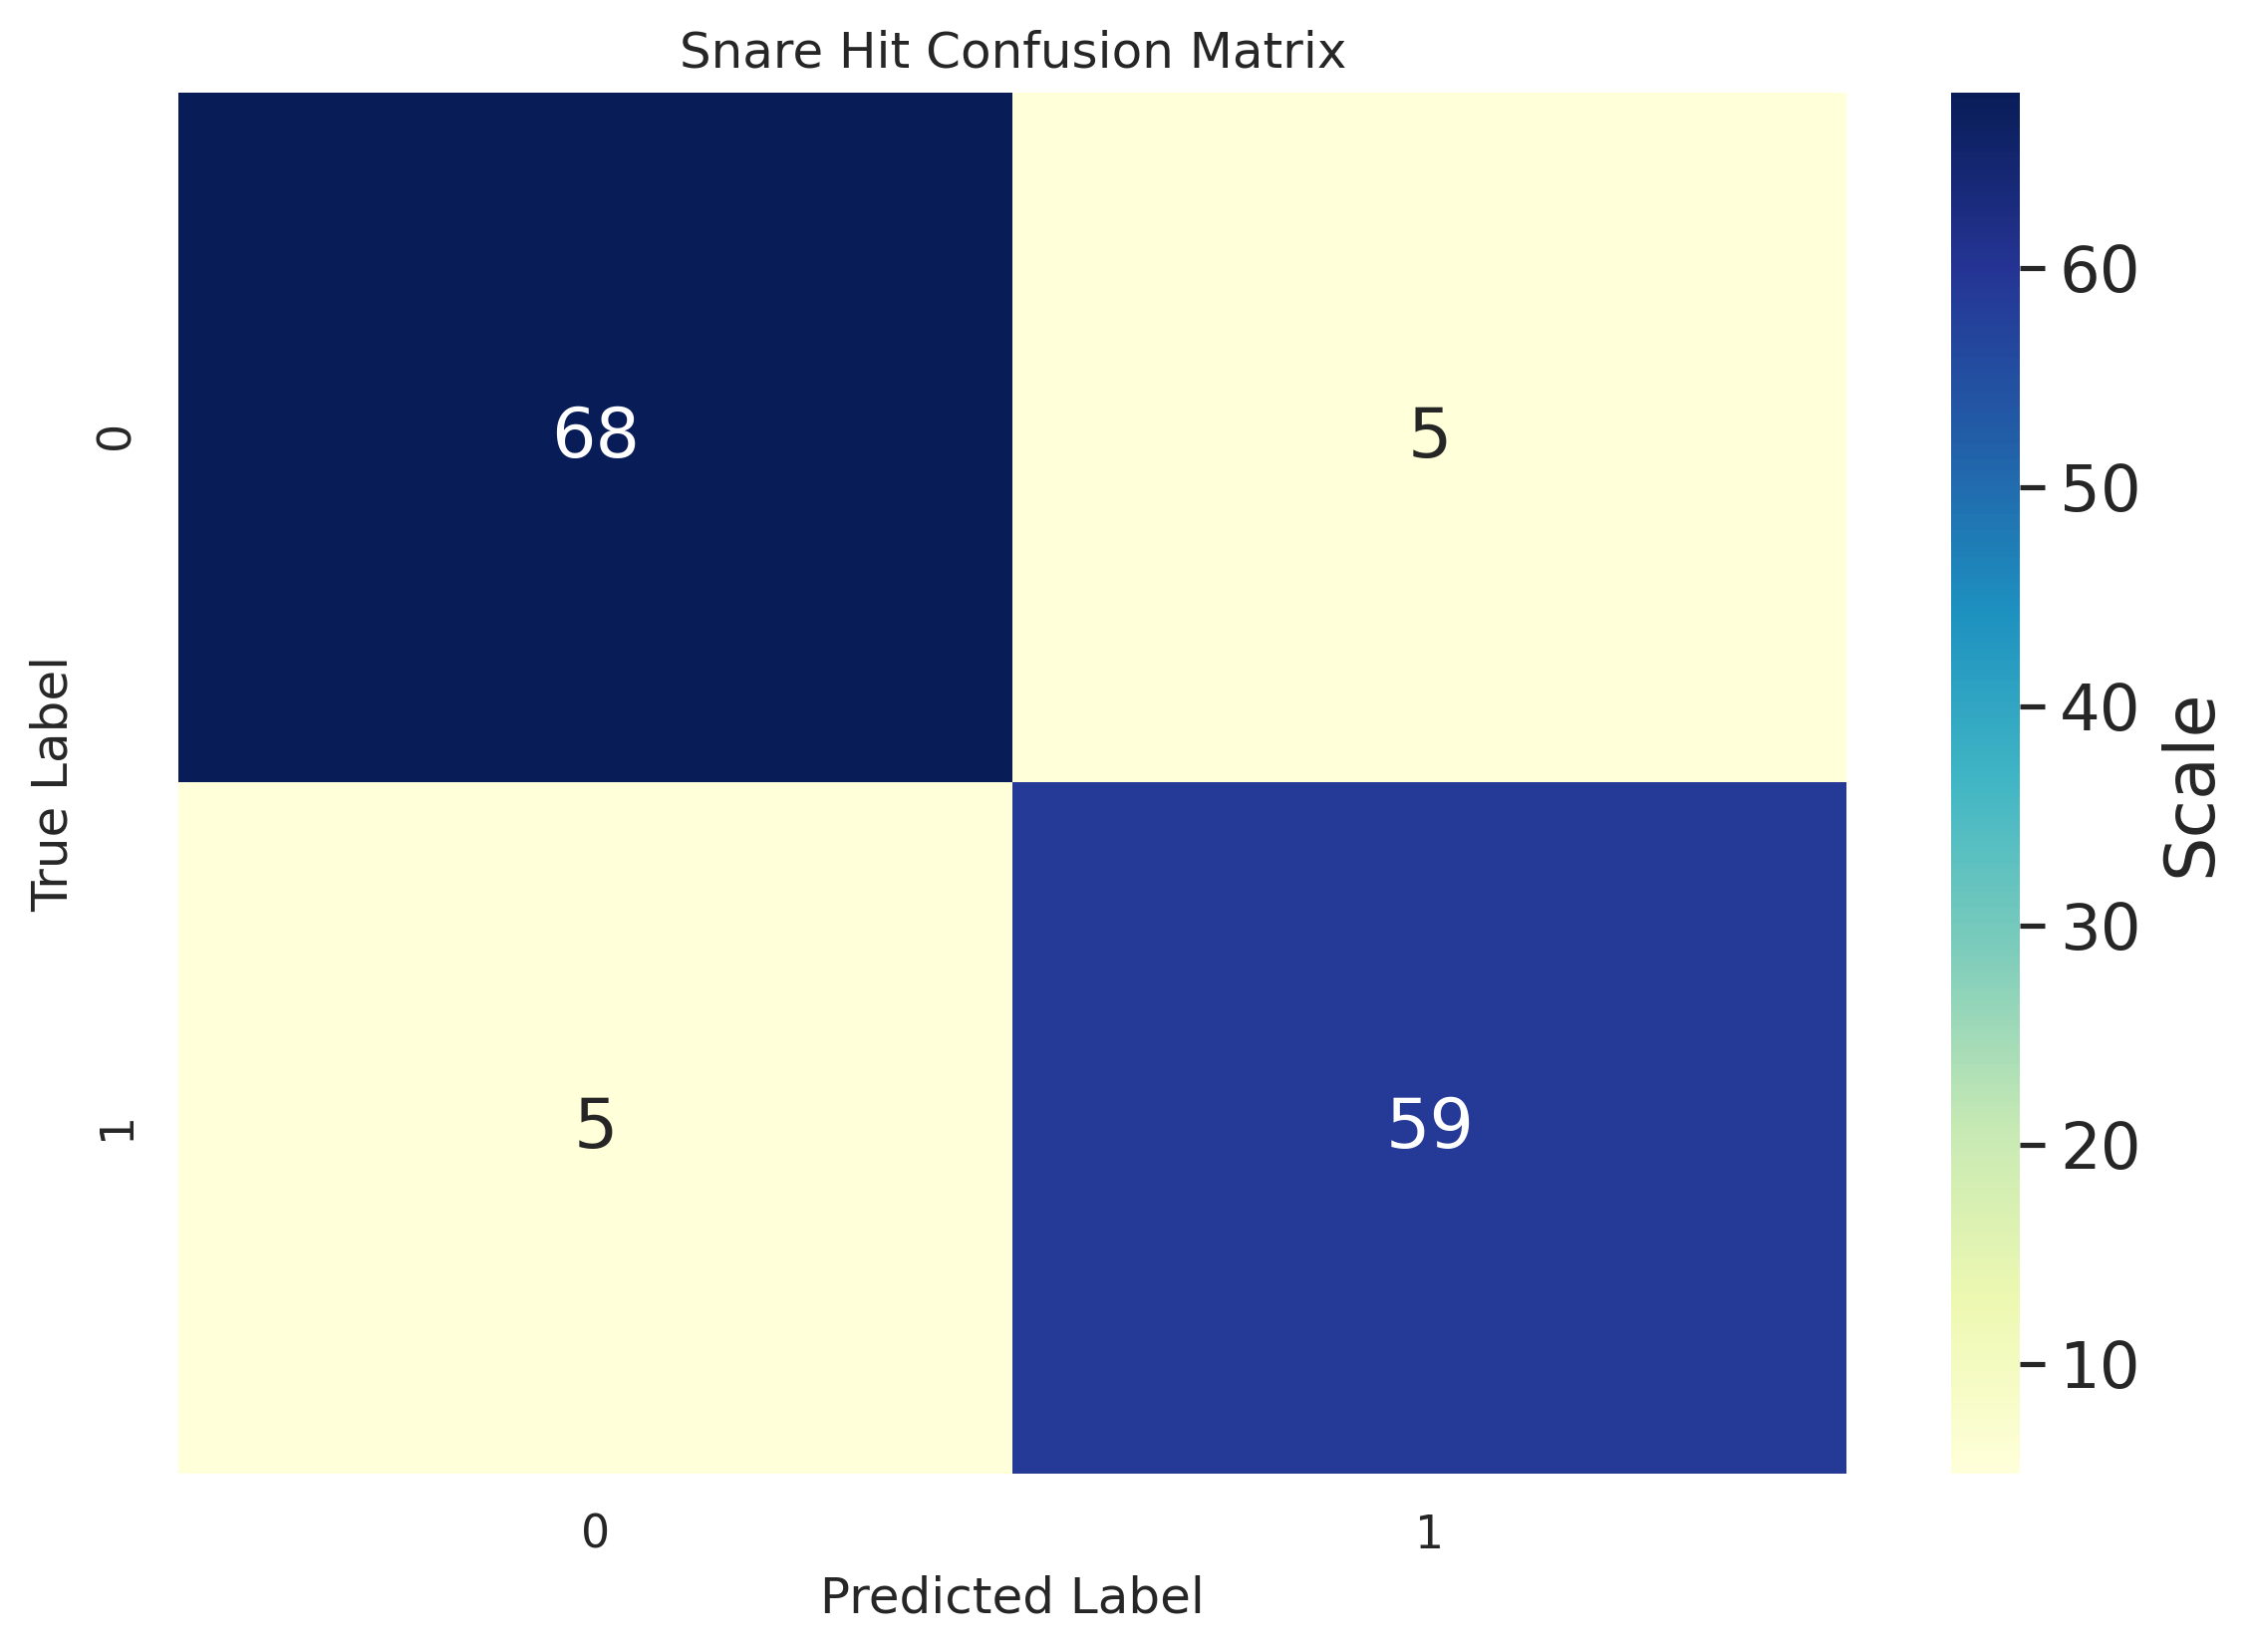
\includegraphics[width=\linewidth]{./immagini/first_classification/sn_hit_cm.png}
		\caption{Matrice di confusione per il colpo di rullante}
		\label{fig:cm_1c}
	\end{subfigure}\hfill
	\begin{subfigure}{.5\linewidth}
		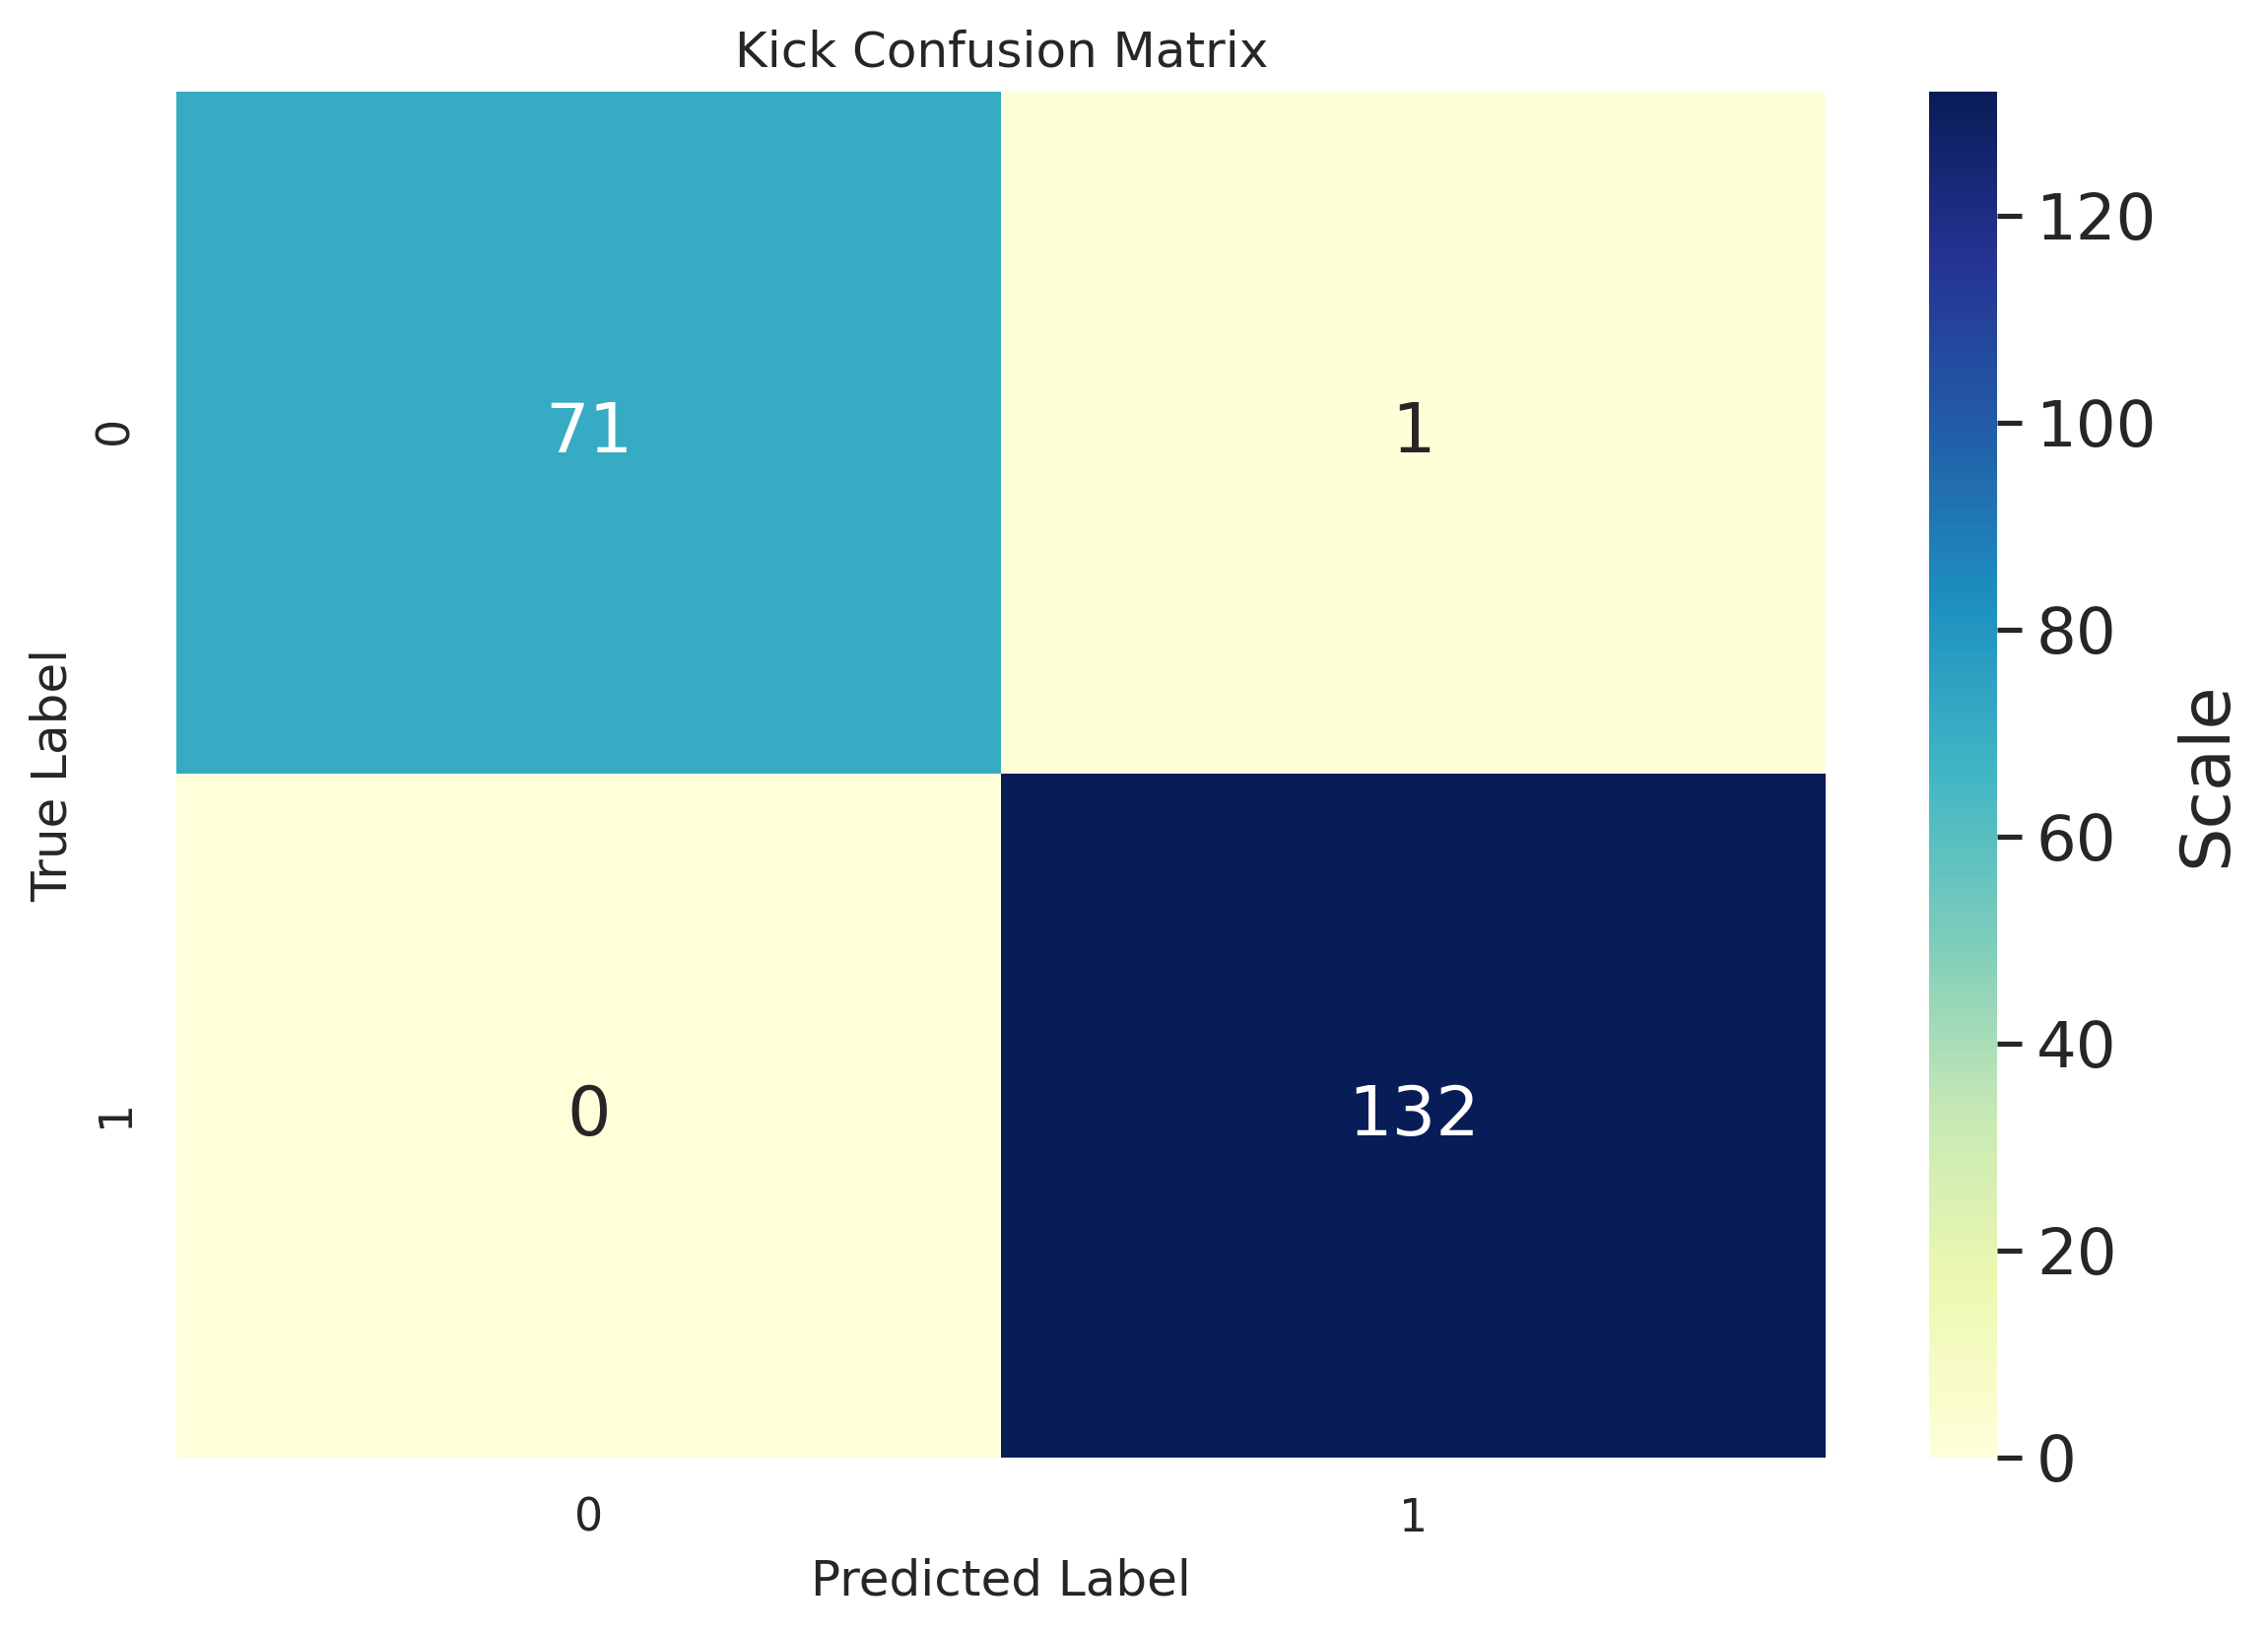
\includegraphics[width=\linewidth]{./immagini/first_classification/kick_cm.png}
		\caption{Matrice di confusione per la cassa}
		\label{fig:cm_1d}
	\end{subfigure}
	\caption{Matrici di confusione della prima fase}
	\label{fig:cm_1}
\end{figure}

Gli esperimenti sono stati condotti alla stessa maniera utilizzando l'approccio di cross validation con un $k=10$ numero di sotto insiemi in cui viene diviso il data-set \ref{proc:cross-validation}.
Osservando dunque numerosità dei dati e i risultati delle matrici di confusione possiamo ora valutare la qualità dei risultati ottenuti calcolando i parametri presentati nel paragrafo \ref{formula:all}.\\

Procedendo per ordine osservando il basso si ha un'accuracy pari a $0.92$ seguita dai valori illustrati nella tabella \ref{tab:cb_res_1}. In seguito sono presenti le misure delle due tipologie di note provocate dal rullante, spazzolato e colpo normale, avneit accuracy rispettivamente di $0.84$ e $0.92$ con i valori presenti nelle tabelle \ref{tab:sn_brush_res_1} e \ref{tab:sn_hit_res_1}. Per quanto riguarda i risultati ottenuti dalla cassa sono un accuracy pari a $0.99$ e la tabella \ref{tab:kick_res_1} mostra i valori a essa relativi.

% Basso
\begin{table}[h!]
	\begin{center}
		\begin{tabular}{l|c|c|c|c|c|r} % <-- Alignments: 1st column left, 2nd middle and 3rd right, with vertical lines in between
			\textbf{Basso} & \textbf{TPR} & \textbf{FPR} & \textbf{Precision} & \textbf{Recall} & \textbf{F-Measure} & \textbf{ROC Area}\\
			%$\alpha$ & $\beta$ & $\gamma$ \\
			\hline
			si & 0,942 & 0,106 & 0,919 & 0,942 & 0,931 & 0,946 \\
			no & 0,894 & 0,058 & 0,923 & 0,894 & 0,908 & 0,946 \\
		\end{tabular}
		\caption{Risultati basso per la prima fase.}
		\label{tab:cb_res_1}
	\end{center}
\end{table}

% Rullante spazzolato
\begin{table}[h!]
	\begin{center}
		\begin{tabular}{l|c|c|c|c|c|r} % <-- Alignments: 1st column left, 2nd middle and 3rd right, with vertical lines in between
			\textbf{Rull. Spazz.} & \textbf{TPR} & \textbf{FPR} & \textbf{Precision} & \textbf{Recall} & \textbf{F-Measure} & \textbf{ROC Area}\\
			%$\alpha$ & $\beta$ & $\gamma$ \\
			\hline
			si & 0,838 & 0,137 & 0,870 & 0,838 & 0,854 & 0,861 \\
			no & 0,863 & 0,163 & 0,163 & 0,863 & 0,846 & 0,861 \\
		\end{tabular}
		\caption{Risultati rullante spazzolato per la prima fase.}
		\label{tab:sn_brush_res_1}
	\end{center}
\end{table}

% Colpo di rullante
\begin{table}[h!]
	\begin{center}
		\begin{tabular}{l|c|c|c|c|c|r} % <-- Alignments: 1st column left, 2nd middle and 3rd right, with vertical lines in between
			\textbf{Rull. Colpo} & \textbf{TPR} & \textbf{FPR} & \textbf{Precision} & \textbf{Recall} & \textbf{F-Measure} & \textbf{ROC Area}\\
			%$\alpha$ & $\beta$ & $\gamma$ \\
			\hline
			si & 0,922 & 0,068 & 0,922 & 0,922 & 0,922 & 0,939 \\
			no & 0,932 & 0,078 & 0,932 & 0,932 & 0,932 & 0,939 \\
		\end{tabular}
		\caption{Risultati colpo di rullante per la prima fase.}
		\label{tab:sn_hit_res_1}
	\end{center}
\end{table}

% Colpo di cassa
\begin{table}[h!]
	\begin{center}
		\begin{tabular}{l|c|c|c|c|c|r} % <-- Alignments: 1st column left, 2nd middle and 3rd right, with vertical lines in between
			\textbf{Cassa} & \textbf{TPR} & \textbf{FPR} & \textbf{Precision} & \textbf{Recall} & \textbf{F-Measure} & \textbf{ROC Area}\\
			%$\alpha$ & $\beta$ & $\gamma$ \\
			\hline
			si & 1,000 & 0,014 & 0,992 & 1,000 & 0,996 & 0,993 \\
			no & 0,986 & 0,000 & 1,000 & 0,986 & 0,993 & 0,993 \\
		\end{tabular}
		\caption{Risultati colpo di cassa per la prima fase.}
		\label{tab:kick_res_1}
	\end{center}
\end{table}

%\begin{table}[h!]
%	\begin{center}
%		\begin{tabular}{l|c|c|r} % <-- Alignments: 1st column left, 2nd middle and 3rd right, with vertical lines in between
%			\textbf{Classe} & \textbf{ACC} & \textbf{TPR} & \textbf{TNR} \\
%			%$\alpha$ & $\beta$ & $\gamma$ \\
%			\hline
%			Basso & 0.92 & 0.94 & 0.90\\
%			Spazzolata di Rullante & 0.85 & 0.84 & 0.86\\
%			Colpo di Rullante & 0.93 & 0.92 & 0.93\\
%			Cassa & 0.99 & 1.00 & 0.99
%		\end{tabular}
%		\caption{Metriche di valutazione prima fase.}
%		\label{tab:accuracy_1}
%	\end{center}
%\end{table}

È possibile notare degli ottimi risultati per tutti gli strumenti nel riconoscimento, in particolar modo per la cassa e il colpo di rullante, vista la natura dell'onda sonora da loro prodotta, un'impulso con una crescita molto rapida sono questi gli strumenti più semplici da riconoscere per la macchina. Lo strumento che è riconosciuto peggio è invece il rullante spazzolato, anch'esso per la natura dell'onda sonora da lui prodotto, meno distinguibile da un possibile rumore per ampiezza d'onda e impulso con crescita molto minore.\\
Essendo questi risultati molto buoni, soprattutto per quanto riguarda la ROC Area, è possibile affermare che con le features utilizzate risulta possibile distinguere tra una nota e una non nota, e dunque passare a una fase di riconoscimento più fine illustrata nella sezione che segue.\\

\section{Seconda fase}
In questa fase si vuole rendere più fine il riconoscimento delle note, consentendo di accettare in input un'intera traccia audio e non solo dei singoli frammenti di note o non per il riconoscimento. Partendo dalla classificazione, viene sempre utilizzato J48 per costruire un albero di decisione che non porterà più a decidere se un frammento analizzato è una nota o meno, questo infatti porterà a classificare in 5 classi diverse ogni elemento di input, come appunto descritto a inizio capitolo. L'algoritmo di classificazione è molto simile al passo precedente, l'unica differenza è che vengono scelti dei campioni più lunghi per poter essere spezzati in più sub-campioni, il primo classificato come 5 (certamente una nota), l'ultimo come 1 (certamente non una nota). Ogni sub-campione avrà la stessa lunghezza, e proprio così facendo è stato possibile fornire in input delle intere tracce, perché suddivise in sub-campioni, di lunghezza costante, al quale si associa a ognuno una classe da 1 a 5 che consente così di localizzare temporalmente le note, e risolvere dunque il problema posto inizialmente.\\
%INSERISCI MATRICI DI CONFUSIONE

\begin{figure}[h!]
	\centering
	\begin{subfigure}{.5\linewidth}
		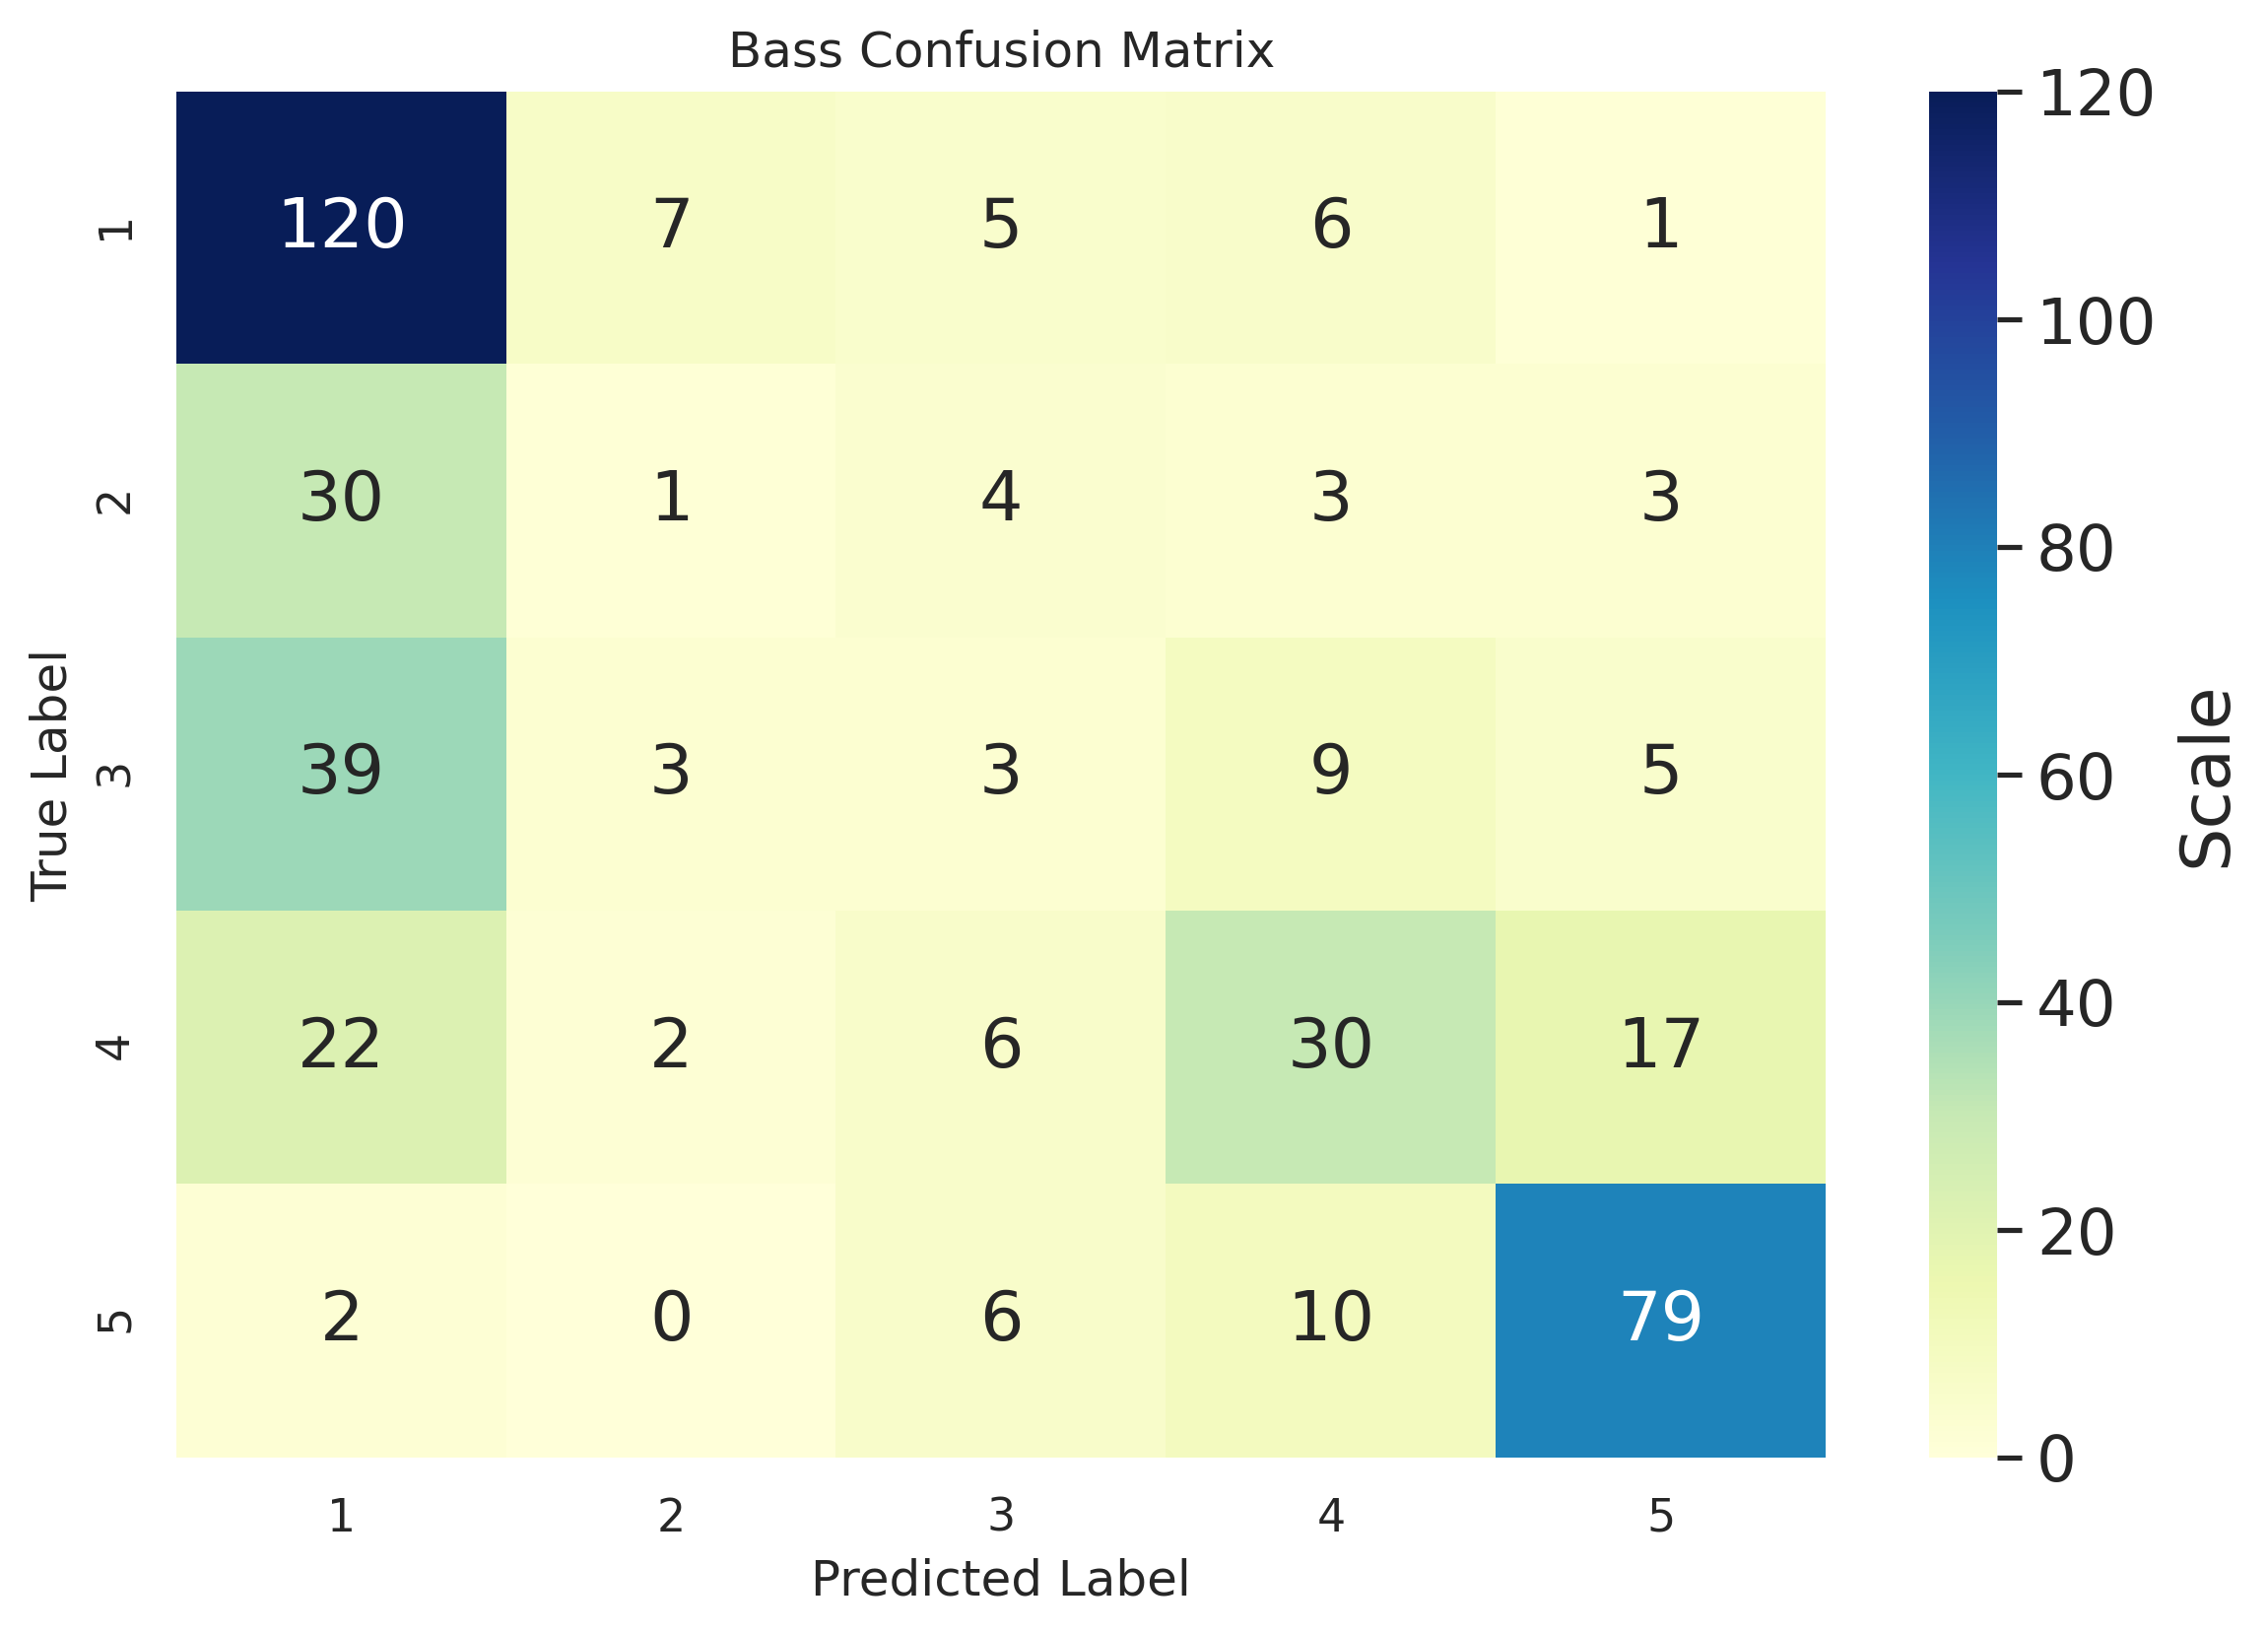
\includegraphics[width=\linewidth]{./immagini/second_classification/cb_cm.png} 
		\caption{Matrice di confusione per il basso}
		\label{fig:cm_2a}
	\end{subfigure}\hfill
	\begin{subfigure}{.5\linewidth}
		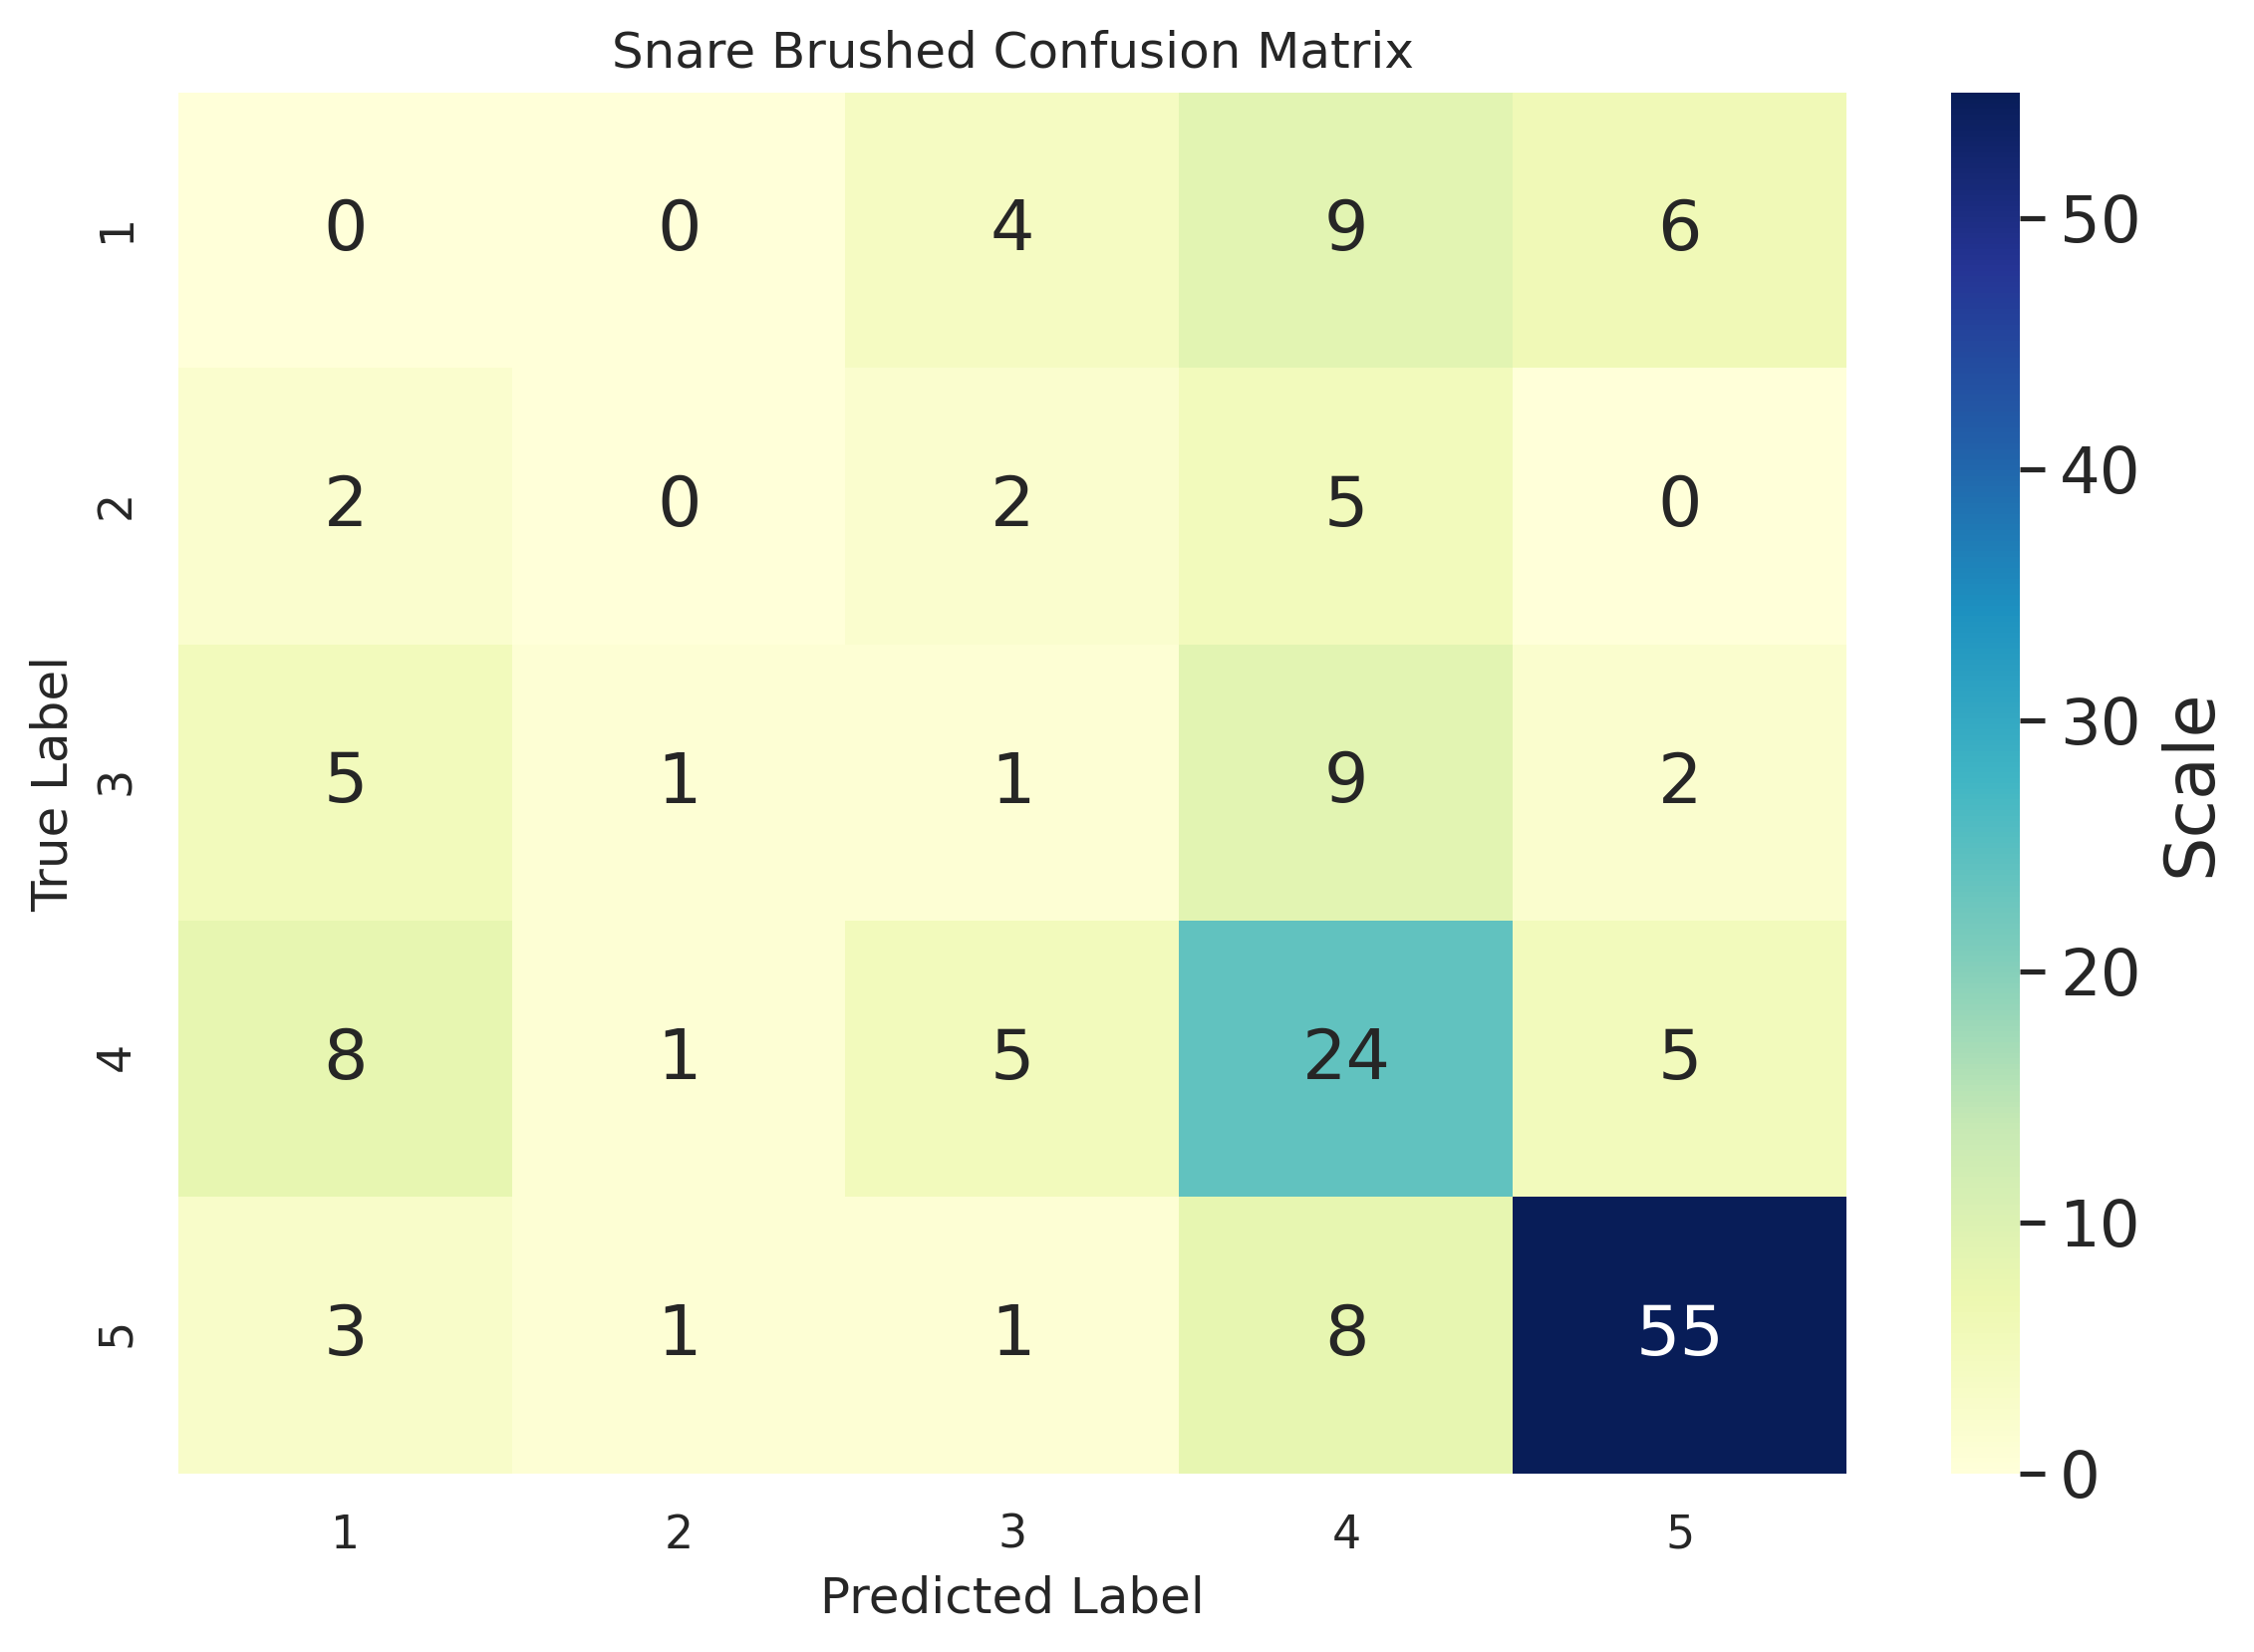
\includegraphics[width=\linewidth]{./immagini/second_classification/sn_brushed_cm.png}
		\caption{Matrice di confusione per il rullante spazzolato}
		\label{fig:cm_2b}
	\end{subfigure}
	
	\begin{subfigure}{.5\linewidth}
		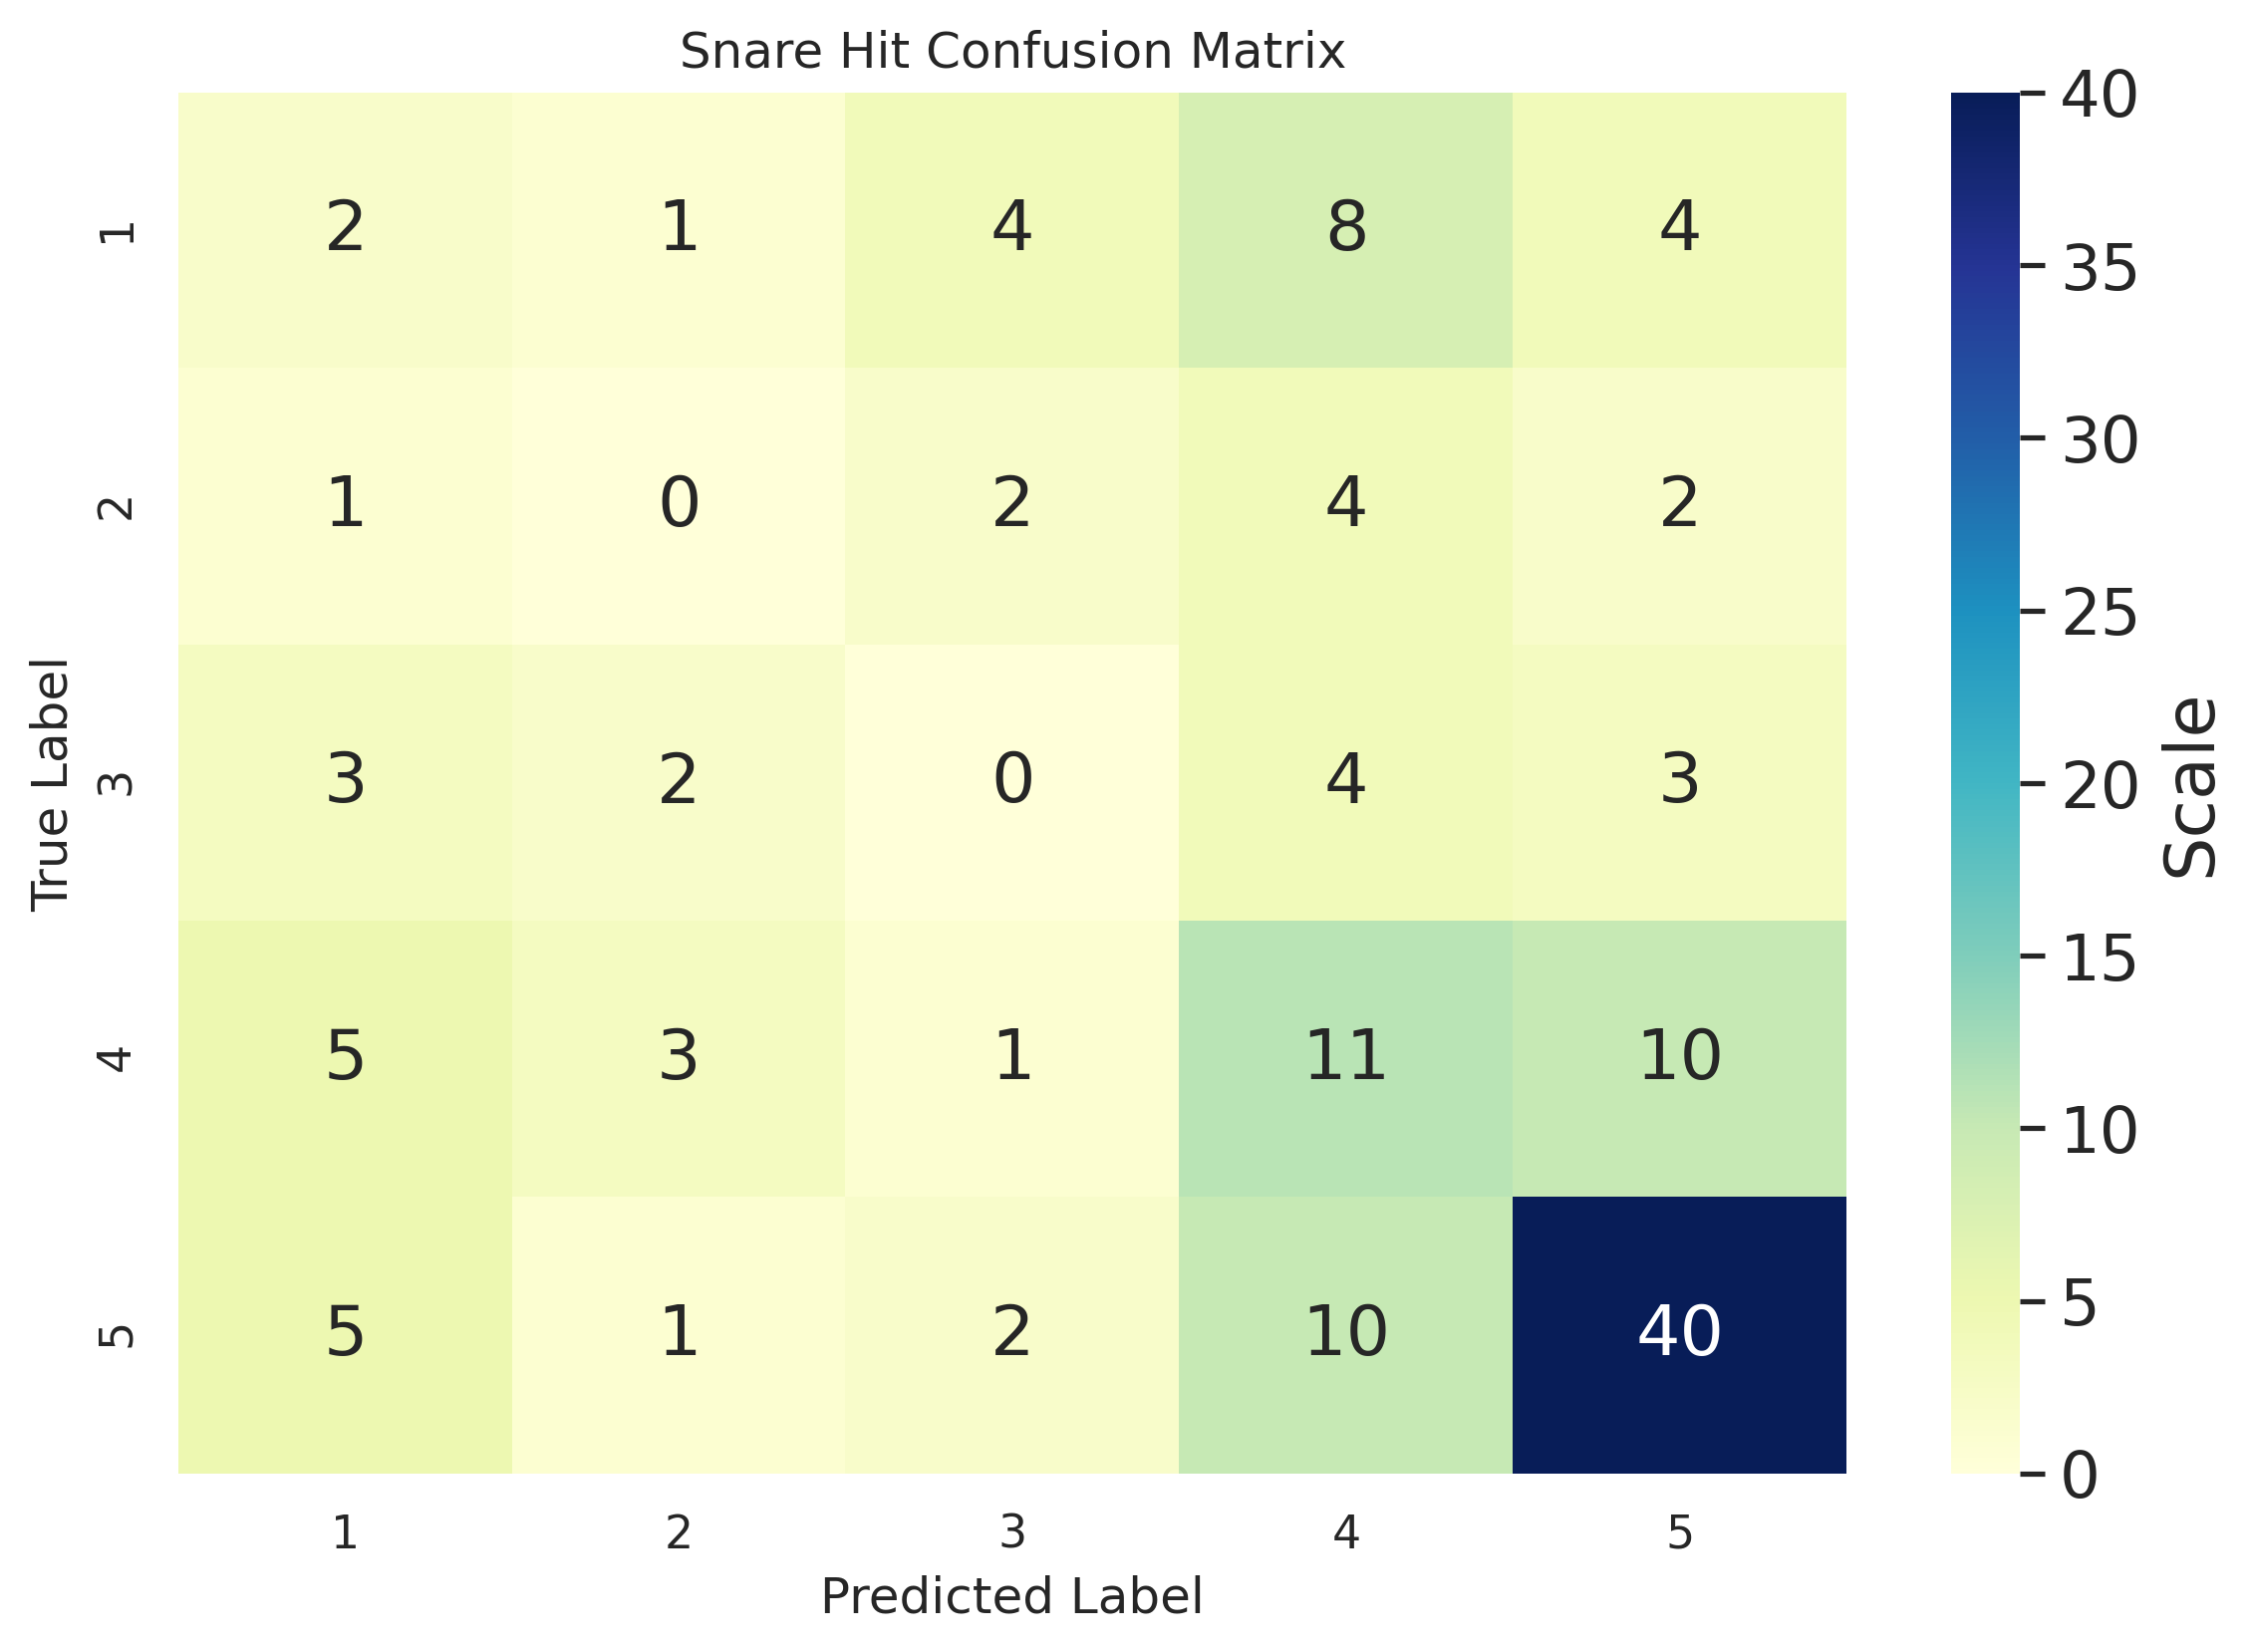
\includegraphics[width=\linewidth]{./immagini/second_classification/sn_hit_cm.png}
		\caption{Matrice di confusione per il colpo di rullante}
		\label{fig:cm_2c}
	\end{subfigure}\hfill
	\begin{subfigure}{.5\linewidth}
		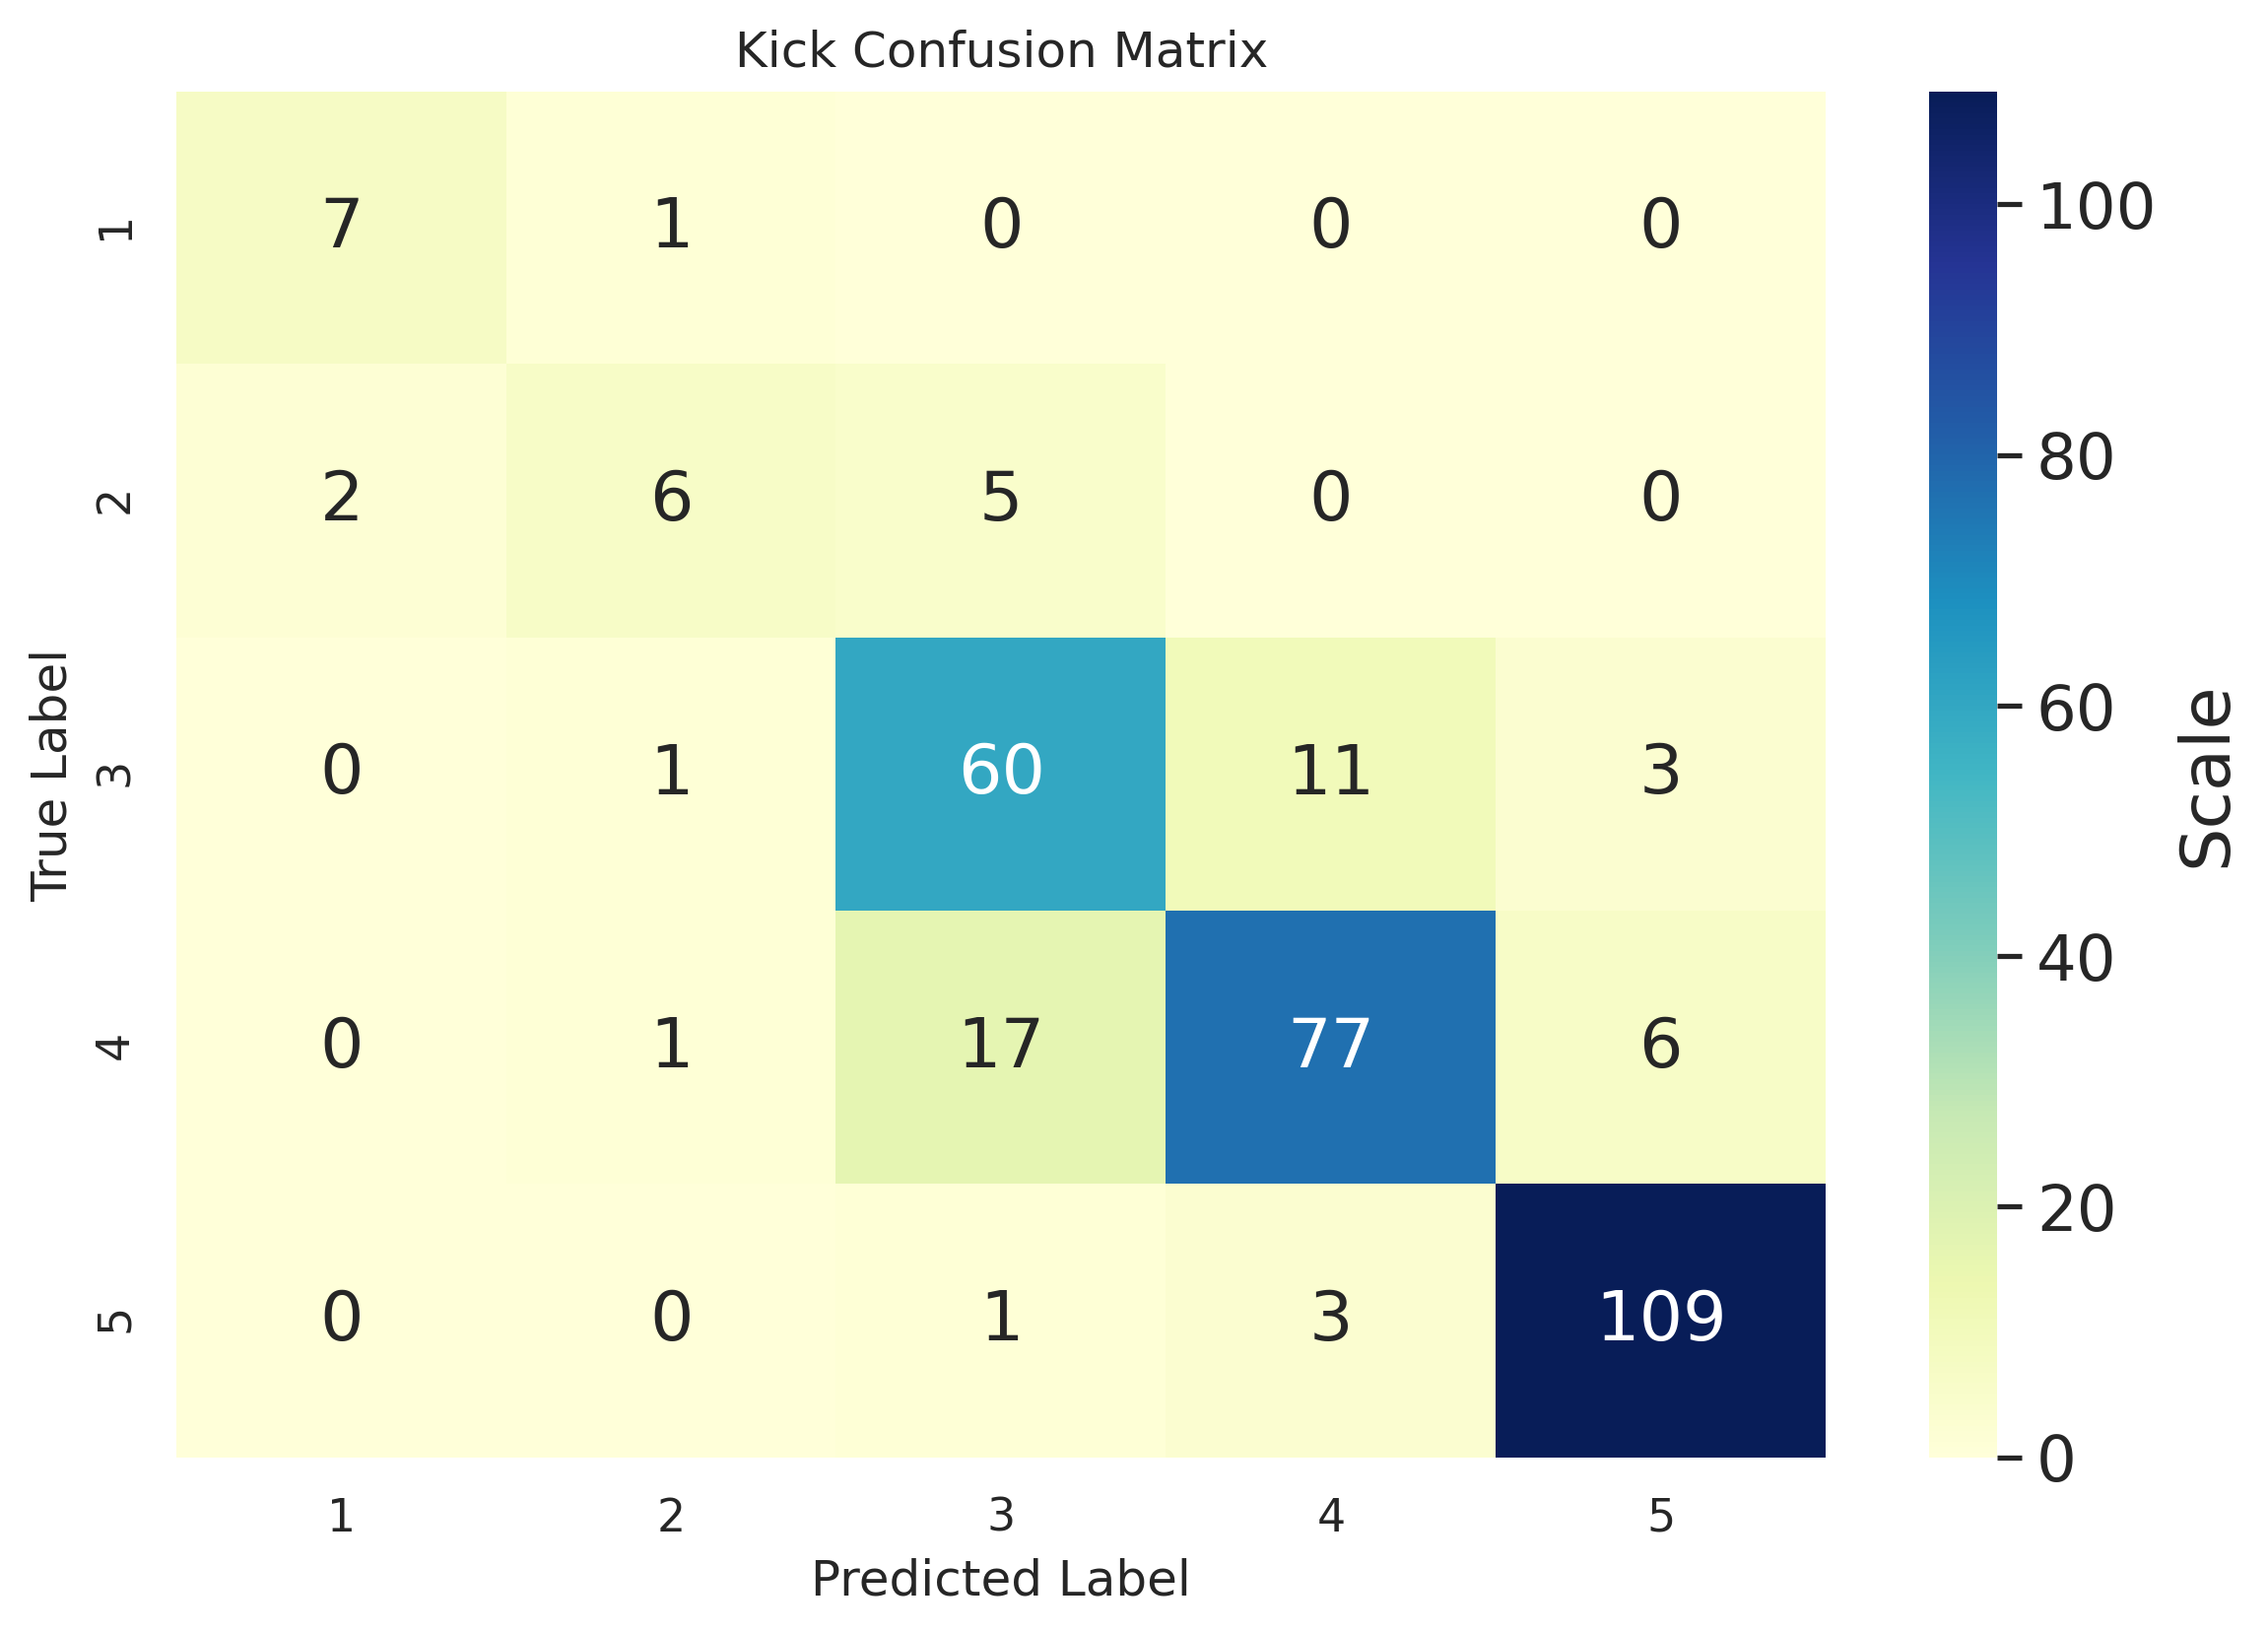
\includegraphics[width=\linewidth]{./immagini/second_classification/kick_cm.png}
		\caption{Matrice di confusione per la cassa}
		\label{fig:cm_2d}
	\end{subfigure}
	\caption{Matrici di confusione della seconda fase}
	\label{fig:cm_2}
\end{figure}

%SPIEGA QUALI SONO I PARAMETRI  CHE INFLUENZANO I RISULTATI, GRANULARITÀ, WINDOW LENGTH E OVERLAP.
Questi risultati sono stati ottenuti effettuando una classificazione dove ogni sub campione è esattamente 8820 campioni, quindi 0.2s, per il campione successivo si esegue uno shift di 4410 campioni, ottenendo 0.1s di granularità e di overlap\footnote{Il tempo di sovrapponimento tra un sub-campione e l'altro}. Anche qui in modo analogo alla prima fase il DT viene condotto l'esperimento con un k=10 numero di sotto-insiemi in cui viene diviso il data-set. Possiamo vedere la numerosità dei campioni selezionati dalle tracce audio nella tabella \ref{tab:numerosità_2.1} e la numerosità delle classi da 1 a 5 per i sub-campioni derivati dai campioni nella tabella \ref{tab:numerosità_2.2}\\

\begin{table}[h!]
	\begin{center}
		\begin{tabular}{l|r} % <-- Alignments: 1st column left, 2nd middle and 3rd right, with vertical lines in between
			\textbf{Classe} & \textbf{Campioni}\\
			%			$\alpha$ & $\beta$ & $\gamma$ \\
			\hline
			Basso & 103\\
			Rullante Spazzolato & 115\\
			Colpo di Rullante & 146\\
			Cassa & 119
		\end{tabular}
		\caption{Numerosità campioni seconda fase.}
		\label{tab:numerosità_2.1}
	\end{center}
\end{table}

\begin{table}[h!]
	\begin{center}
		\begin{tabular}{l|c|c|c|c|r} % <-- Alignments: 1st column left, 2nd middle and 3rd right, with vertical lines in between
			\textbf{Classe} & \textbf{1} & \textbf{2} & \textbf{3} & \textbf{4} & \textbf{5}\\
			%			$\alpha$ & $\beta$ & $\gamma$ \\
			\hline
			Basso & 139 & 41 & 59 & 77 & 97\\
			Rullante Spazzolato & 19 & 9 & 18 & 43 & 68\\
			Colpo di Rullante & 20 & 9 & 13 & 30 & 58\\
			Cassa & 8 & 13 & 75 & 101 & 113
		\end{tabular}
		\caption{Numerosità campioni seconda fase.}
		\label{tab:numerosità_2.2}
	\end{center}
\end{table}

I numeri dei campioni audio selezionati nella prima tabella sono molto omogenei, ma data la natura delle registrazioni e degli strumenti oltre al modo in cui questi vengono suonati porta ad avere nella seconda tabella valori molto eterogenei di sub-campioni per ogni classe. Osserviamo infatti che il per il basso e la cassa si possiedono il maggior numero di sub-campioni a differenza delle due tipologie di rullanti, con un numero molto minore a confronto. Il rullante è uno strumento che in questo contesto produce note molto ravvicinate tra loro e per questo motivo molti campioni non possono essere usati perché troppo corti rispetto alla dimensione che è stata utilizzata per l'esperimento, lo stesso vale per i sotto campioni, questi infatti sono molto meno dal momento che effettuando dei tagli di campioni che già di natura sono corti, il risultato è di conseguenza un numero inferiore di sotto-campioni, in particolar modo appartenenti alla classe ``1'', maggiore è il numero invece per la classe ``5'', appunto per come vengono etichettati si sub-campioni.\\

I risultati ottenuti mostrano un'accuracy pari a 0.56 per il basso, un valore molto inferiore rispetto al risultato più che positivo ottenuto nella prima fase. La tabella \ref{tab:cb_res_2} ci mostra in modo più preciso che cosa succede per le singole classi, da subito si possono notare dei risultati molto positivi nel riconoscimento delle classi 5 e 1 con dei TPR vicini a 0.9, accompagnati da valori positivi, anche rispetto a quelli delle altre classi d ROC Area. La prestazione peggiore è osservata invece per la classe 3, sembra che crei molta confusione per il riconoscimento.
I risultati analizzati in seguito sono quelli del rullante spazzolato, e del colpo di rullante, i risultati peggiori in assoluto in questo set di strumenti con accuracy rispettivamente di 0.50 e 0.41, questa imprecisione molto elevata è probabile che sia originata dal modo in cui vengono estratti i campioni, oltre agli aspetti definiti nella prima fase. Le rispettive tabelle \ref{tab:sn_brush_res_2} e \ref{tab:sn_hit_res_2} mostrano in modo molto chiaro il peggioramento, ma solo per alcune classi. Partendo dal TPR di tutte e due si può evincere l'incapacità della macchina nel riconoscere le classi 1 e 2, questo probabilmente dato da numero di sub-campioni troppo piccolo, come anche dalla natura del suono da esso generato nella prima fase. Quello che è però il TPR delle classi 5 dei due rullanti, si vede un miglioramento, in particolar modo per quanto riguarda il rullante spazzolato, con un valore che si avvicina molto di più a 1 di quanto le altre classi non facciano. Per comprendere meglio la qualità dei classificatori ottenuti consideriamo la ROC Area, che per la classe 5 del rullante spazzolato ha un valore molto buono, che va però a scendere con lo scendere delle classi. In modo simile si comporta il classificatore per il colpo di rullante, con la differenza però che la classe con il risultato peggiore è la 3.
In fine per quanto riguarda la cassa è stato ottenuto un risultato più che positivo con un valore di accuracy pari a 0.83, il valore migliore per questa fase, accompagnato da metriche di valutazione molto buone presentate nella tabella \ref{tab:kick_res_2} partendo da un valore di TPR molto buono per la classe, leggermente inferiore per le altre, con un esito invece non ideale nella classe 2. Portiamo maggiore attenzione alla ROC area, con valori molto vicini a 1, mostrando che il classificatore ottenuto è in grado di lavorare molto bene. Anche in questo caso influiscono, però positivamente, le caratteristiche dell'onda sonora prodotta dalla cassa discusse precedentemente.\\


% Basso
\begin{table}[h!]
	\begin{center}
		\begin{tabular}{l|c|c|c|c|c|r} % <-- Alignments: 1st column left, 2nd middle and 3rd right, with vertical lines in between
			\textbf{Basso} & \textbf{TPR} & \textbf{FPR} & \textbf{Precision} & \textbf{Recall} & \textbf{F-Measure} & \textbf{ROC Area}\\
			%$\alpha$ & $\beta$ & $\gamma$ \\
			\hline
			1 & 0,863 & 0,339 & 0,563 & 0,863 & 0,682 & 0,790 \\
			2 & 0,024 & 0,032 & 0,077 & 0,024 & 0,037 & 0,604 \\
			3 & 0,051 & 0,059 & 0,125 & 0,051 & 0,072 & 0,609 \\
			4 & 0,390 & 0,083 & 0,517 & 0,390 & 0,444 & 0,676 \\
			5 & 0,814 & 0,082 & 0,752 & 0,814 & 0,782 & 0,890
		\end{tabular}
		\caption{Risultati basso per la seconda fase.}
		\label{tab:cb_res_2}
	\end{center}
\end{table}

% Rullante spazzolato
\begin{table}[h!]
	\begin{center}
		\begin{tabular}{l|c|c|c|c|c|r} % <-- Alignments: 1st column left, 2nd middle and 3rd right, with vertical lines in between
			\textbf{Rull. Spazz.} & \textbf{TPR} & \textbf{FPR} & \textbf{Precision} & \textbf{Recall} & \textbf{F-Measure} & \textbf{ROC Area}\\
			%$\alpha$ & $\beta$ & $\gamma$ \\
			\hline
			1 & 0,000 & 0,130 & 0,000 & 0,000 & 0,000 & 0,479 \\
			2 & 0,000 & 0,020 & 0,000 & 0,000 & 0,000 & 0,531 \\
			3 & 0,056 & 0,086 & 0,077 & 0,056 & 0,065 & 0,509 \\
			4 & 0,558 & 0,272 & 0,436 & 0,558 & 0,490 & 0,695 \\
			5 & 0,809 & 0,146 & 0,809 & 0,809 & 0,809 & 0,856 \\
		\end{tabular}
		\caption{Risultati rullante spazzolato per la seconda fase.}
		\label{tab:sn_brush_res_2}
	\end{center}
\end{table}

% Colpo di rullante
\begin{table}[h!]
	\begin{center}
		\begin{tabular}{l|c|c|c|c|c|r} % <-- Alignments: 1st column left, 2nd middle and 3rd right, with vertical lines in between
			\textbf{Rull. Colpo} & \textbf{TPR} & \textbf{FPR} & \textbf{Precision} & \textbf{Recall} & \textbf{F-Measure} & \textbf{ROC Area}\\
			%$\alpha$ & $\beta$ & $\gamma$ \\
			\hline
			1 & 0,105 & 0,128 & 0,125 & 0,105 & 0,114 & 0,556 \\
			2 & 0,000 & 0,059 & 0,000 & 0,000 & 0,000 & 0,536 \\
			3 & 0,000 & 0,078 & 0,000 & 0,000 & 0,000 & 0,388 \\
			4 & 0,367 & 0,265 & 0,297 & 0,367 & 0,328 & 0,505 \\
			5 & 0,690 & 0,271 & 0,678 & 0,690 & 0,684 & 0,693 \\
		\end{tabular}
		\caption{Risultati colpo di rullante per la seconda fase.}
		\label{tab:sn_hit_res_2}
	\end{center}
\end{table}

% Colpo di cassa
\begin{table}[h!]
	\begin{center}
		\begin{tabular}{l|c|c|c|c|c|r} % <-- Alignments: 1st column left, 2nd middle and 3rd right, with vertical lines in between
			\textbf{Cassa} & \textbf{TPR} & \textbf{FPR} & \textbf{Precision} & \textbf{Recall} & \textbf{F-Measure} & \textbf{ROC Area}\\
			%$\alpha$ & $\beta$ & $\gamma$ \\
			\hline
			1 & 0,875 & 0,007 & 0,778 & 0,875 & 0,824 & 0,996 \\
			2 & 0,462 & 0,010 & 0,667 & 0,462 & 0,545 & 0,898 \\
			3 & 0,800 & 0,098 & 0,723 & 0,800 & 0,759 & 0,899 \\
			4 & 0,762 & 0,067 & 0,846 & 0,762 & 0,802 & 0,910 \\
			5 & 0,965 & 0,046 & 0,924 & 0,965 & 0,944 & 0,972 \\
		\end{tabular}
		\caption{Risultati colpo di cassa per la seconda fase.}
		\label{tab:kick_res_2}
	\end{center}
\end{table}


A questo punto si hanno due classificatori, uno utilizzato nella prima fase, e uno per la seconda. I risultati ottenuti nella prima fase sono più che positivi, mostrano un approccio  al problema corretto, a differenza della seconda fase. Questa seconda è stata trattata come un problema di classificazione, probabilmente un approccio non sufficientemente adeguato al tipo di problema considerato tanto quanto lo sarebbe un approccio per regressione.
%Dal momento che l'interesse è nel riuscire a collocare temporalmente le note suonate da uno strumento, la classe 5 è quella più importante di tutte, e la stessa ci permette di dire che questo primo approccio se sviluppato ulteriormente potrebbe portare a risultati molto migliori nel tempo, visti quelli ottenuti fino ad'ora. Questo è un approccio sicuramente perfezionabile e non perfetto, ma in grado di fornire dei primi risultati con una granularità al decimo di secondo. 
Oltre a migliorare il riconoscimento, uno degli obiettivi è di portare la granularità al millesimo di secondo in futuro, dal momento che in musica, quelli che sono intervalli di tempo per noi brevi, come 1/10 di secondo, troppo ampi, all'interno di essi possono occorrere un numero molto elevato di eventi. Gli strumenti che sono ritenuti interessanti per gli studi da condurre sono principalmente il basso e la cassa, che come visto, vengono riconosciuti in modo discreto, il rullante, soprattutto quello spazzolato portano delle difficoltà non indifferenti che devono essere superate.\\
Avendo a questo punto un sistema funzionante, il passo successivo è stato la costruzione di una \emph{graphical user interface} (GUI) presentata nel capitolo seguente.

%Nei risultati ottenuti è possibile notare un peggioramento delle predizioni in modo particolare nel rullante, precisamente con un 51\% di istanze classificate correttamente per il rullante spazzolato e un 41\% per il colpo semplice di rullante. Con la cassa è stato ottenuto invece quello che è il risultato migiore con l'83\% di istanze classificate in modo corretto. Questa così ampia divergenza, così come per i risultati ottenuti precedentemente, è data dalla forma e dell'onda sonora in se. Infatti la cassa genera un onda con transiente molto marcato, e facilmente riconoscibile con le features utilizzate, che decade in modo molto rapido differentemente da quanto invece succede con il rullante, in particolar modo quello spazzolato. Un altro aspetto che influisce sull'abilità di riconoscere o meno un'onda sonora da un rumore è dato dall'intensità del segnale generato, infatti il rullante spazzolato genera un'onda con un ampiezza molto inferiore, difficilmente distinguibile da quello che è il rumore. L'ultimo aspetto ma non meno importante riguarda come sono stati selezionati i campioni per allenare la macchina, la numerosità dei campioni estratti e la qualità delle registrazioni utilizzate, tutti questi parametri possono influenzare pesantemente quelli che sono i risultati. Un numero maggiore di campioni potrebbe insegnare in modo migliore alla macchina la quale sarà in grado di costruire un albero di decisione migliore, come anche delle registrazioni migliori o con  volumi maggiori per alcuni strumenti dove possibile.